% ---------------------------------------------------------------------
% EG author guidelines plus sample file for EG publication using LaTeX2e input
% D.Fellner, v1.17, Sep 23, 2010


\title[Automatic Proxy Geometry]%
      {Automatic Proxy Geometry}

% for anonymous conference submission please enter your SUBMISSION ID
% instead of the author's name (and leave the affiliation blank) !!
\author[J.\,O. Nygaard \& J. Mikkelsen]
       {J.\,O. Nygaard$^{1}$
        and J. Mikkelsen$^{1}$
        and Husk Anonymisering Hvis Paakrevet!$^{1}$
%        S. Spencer$^2$\thanks{Chairman Siggraph Publications Board}
        \\
% For Computer Graphics Forum: Please use the abbreviation of your first name.
         $^1$SINTEF ICT, applied mathematics, Norway
%        $^2$ Another Department to illustrate the use in papers from authors
%             with different affiliations
       }

% ------------------------------------------------------------------------

% if the Editors-in-Chief have given you the data, you may uncomment
% the following five lines and insert it here
%
% \volume{27}   % the volume in which the issue will be published;
% \issue{1}     % the issue number of the publication
% \pStartPage{1}      % set starting page


%-------------------------------------------------------------------------
\begin{document}

% \teaser{
%  \includegraphics[width=\linewidth]{eg_new}
%  \centering
%   \caption{New EG Logo}
% \label{fig:teaser}
% }

\maketitle

\begin{abstract}
   We describe an algorithm, and implementation, of an automatic proxy geometry
   system for a server-client remote rendering setup. The client may be a thin
   client in the form of a hand-held pad, for our implementation we only assume
   the availability of WebGL. For our rendering server, we make use of a
   GL-capable web server. In situations where the rate of received images
   deteriorate due to low bandwith, high latency or long rendering times, the
   client displays an automatically generated proxy geometry. This proxy
   geometry is computed from depth buffers bundled with rendered images from the
   server.
   % Husk: Skal vaere en blank linje nedenfor

\begin{classification} % according to http://www.acm.org/class/1998/
\CCScat{FIX THIS Computer Graphics}{I.3.3}{Picture/Image Generation}{Line and curve generation}
\end{classification}

\end{abstract}




%-------------------------------------------------------------------------
\section{Notes}

\begin{itemize}

\item We restrict ourselves to discuss ``splat sets'' in this paper. (Nevne der det
tas frem andre alternativer)

\item
Husk aa faa med det viktige i at vi faar oekt serverkapasiteten til aa
serve flere klienter ogsaa!

\item
``server-image'' i steden for ``server-rendered image'' for aa spare plass?

\item received stavekontroll

\item Hvor passer det aa faa inn 1) bilde og 2) tekst om FRView?

\item Maa ta et lite soek paa prior art innen omraadet

\end{itemize}

%-------------------------------------------------------------------------
\section{Introduction}

With increasingly powerful rendering engines, in forms ranging from mobile and
hand-held devices to traditional stationary computers, one might be led to
believe that rendering frame rates could only increase and visualization could
only become more interactive. Alas, hand in hand with this development we also
find ever increasing requirements on computation accuracy, power efficiency,
data sizes and so on.

One result of this is that server-side rendering is as relevant as ever
before. And, with a client-server model for rendering, the problems with
transferring images from the server to the model is of course also still
present.

In order to obtain the frame rates on the client suitable for interactive
visualizations, demands are put on bandwidth, latency and rendering speed. If
one or more of these demands are not met, according to a suitable measure, the
frame rate will deteriorate together with the user experince.

One way to deal with such situations is for the client to have a so-called proxy
model, which is defined as a temporary model to be shown and manipulated locally
on the client while waiting for the appropriate image from the server.

A particularly unwelcomed chore is that of building proxy geometries for various
data sets. The typical ``hello world'' proxy geometry is the familiar bounding
box wire frame, but this will degrade the user experience unacceptably for most
applications. One alternative is to hand-build such simpler proxy
geometries. They have to be simple both for the building cost, and also for the
actual rendering on the possibly very thin client. Another alternative is to
automate this process, a large triangulation may for instance be represented by
a much coarser approximating triangulation that can be built automatically. One
disadvantage of this approach is that this is not easy to do for many kinds of
data. 

Our suggested solution is to pass along depth information from the server along
with ordinary rendered images. From this depth image, a rudimentary 3D model can
be built, and using the ordinary image as a texture, this model can be
transformed and rendered on the client while waiting for the next update from
the server. If the server does not take too long to respond, and/or the client
does not change the position or orientation of the model too much, it is to be
hoped that this display of a proxy model integrates seemlessly with the slower
stream of server-rendered frames.

[Kanskje ha inn en foreløpig figur-skisse her, med dybdefelt vist som en
  høydeflate...?]

[Trenger referanser til state of the art o.l. her]

%-------------------------------------------------------------------------

\section{The auto proxy algorithm}

The first main idea is to automatically construct a proxy geometry on the client
side from depth data provided by the server. For a new frame to be displayed on
the client, the server renders an image in a frame buffer, and it is assumed
that it in this process also renders a corresponding depth buffer. This depth
buffer may be regarded as a height map over a viewing plane relative to the
observing client. Hence, this depth map does not contain information about scene
elements not in view for the set of view parameters at the time of server side
rendering. Our approach is based on the assumption that small transformations of
this height map still will give good approximations to the scene being
rendered. These renderings are exactly what the client will compute and show
while waiting for the next update from the server. See
Figure~\ref{fig:2Dheightmap} and Figure~\ref{fig:2DheightmapRoated} for an
illustration of this heightmap computed on the server, and a recovered 3D model
on the client.

\begin{figure}[htb]
  \centering
  \begin{tikzpicture}[scale=0.5, >=triangle 45] % , show background rectangle]


%  \node[scale=0.15, above right] (screenshotcenter) at (0,0) {\includegraphics{test.jpg}};
%  \coordinate (widthheight) at ($2*(screenshotcenter)$);

%  \draw [fill, circle, inner sep=0pt, minimum size=3pt, color=black] (0, 0) circle (3pt);
%  \draw [fill, circle, inner sep=0pt, minimum size=3pt, color=red] (screenshotcenter) circle (3pt);

%  \draw let
%    \p1 = ( $ 2*(screenshotcenter) $ )
%  in
%    [fill=none] (0, 0) rectangle (\x1, \y1);


%  \newcommand\expansion{0.5}
%  \coordinate (lowerleft)        at ( $ (0, 0) - \expansion*(widthheight) $ );
%  \coordinate (upperright)       at ( $ (widthheight) + \expansion*(widthheight) $ );
  
%  \draw [fill=none] (lowerleft) rectangle (upperright);

  % View frustum
  \fill[fill=gray!10] (1, 0.7) -- (9, 0.7) -- (10, 4.3) -- (0, 4.3) -- cycle;

  % Some scene
  \draw[red, line width=3pt] (2, 3) -- (5, 2);
  \draw[green, line width=3pt] (5, 2) -- (8, 4);


  % Corresponding pixels and depth fragments
  \def \pixelwidth  {0.4}
  \def \pixelheight {0.3}
  \def \redstart    {2.2}
  \def \redpixels   {7}
  \def \pixels      {13}
  \foreach \s in {1, ..., \pixels} {
    \def \x { \redstart + \s * \pixelwidth }
    \def \xx { \x + \pixelwidth }
    \ifthenelse{\s < \redpixels} {
      \draw[red, fill=red!50] (\x, 1) rectangle (\xx, 1+\pixelheight); 
    } {
      \draw[green, fill=green!50] (\x, 1) rectangle (\xx, 1+\pixelheight);
    }
    \pgfmathsetmacro\depthcol{abs(\redpixels-0.5-\s) * 25}
    \draw[black, fill=gray!\depthcol] (\x, 1+\pixelheight) rectangle (\xx, 1+2*\pixelheight);
  }


%\def \n {5}
%\def \radius {3cm}
%\def \margin {8} % margin in angles, depends on the radius
%\foreach \s in {1,...,\n}
%{
%  \node[draw, circle] at ({360/\n * (\s - 1)}:\radius) {$\s$};
%  \draw[->, >=latex] ({360/\n * (\s - 1)+\margin}:\radius) 
%    arc ({360/\n * (\s - 1)+\margin}:{360/\n * (\s)-\margin}:\radius);
%}



  % Indicated nodes and intersections
%  \draw [fill, circle, inner sep=0pt, minimum size=3pt, color=black] (T0) circle (3pt);

  % Labels
%  \draw (T0) node[black, scale=0.8, shift={(0, -2ex)}] {$\Tv_0$};


\end{tikzpicture}

  \caption{\label{fig:2Dheightmap}
           The rendered image (of \eg, a cube) as a height map seen from above,
           for a certain transformation. \textbf{Droppe denne?}}
\end{figure}

\begin{figure}[htb]
  \centering
  \subfigure[Low frame rate]{
    %\begin{tikzpicture}[ scale=.25, show background rectangle]
\begin{tikzpicture}[scale=0.32, >=triangle 45, show background rectangle,
  declare function = {
    rotx(\x,\y,\th) = cos(\th)*\x - sin(\th)*\y; % NB! Cannot have space between parameters it seems!
    roty(\x,\y,\th) = sin(\th)*\x + cos(\th)*\y;
  }
  ]

  % View frustum
  \fill[fill=gray!20] (1, 0) -- (9, 0) -- (10, 5) -- (0, 5) -- cycle;
  % \clip (1, 0) -- (9, 0) -- (10, 5) -- (0, 5) -- cycle;
  % Clipping looks ok, but clipped content still expands bbox!! Solving this by reducing \pixels below from 13 to 11...


  % Defining some figure params

  \def \pixelwidth  {0.4}
  \def \pixelheight {0.3}
  \def \redstart    {2.2}
  \def \redpixels   {5}
  \def \pixels      {11}
  \def \linewidth   {1.25pt}
  \def \theta       {25}
  \def \cx          {5}
  \def \cy          {3}
  \def \rightcol    {red!100}
  \def \leftcolL    {blue!100}
  %\def \leftcolR    {red!100!blue!0} % Why doesn't this work?! (The color becomes white)
  \def \leftcolR    {red!100}


  % The scene, using same coordinate calculations as in the loop below

  \foreach \t in {0, ..., 4} {

    \pgfmathsetmacro\theta{25*\t}

    \ifthenelse{ \t = 0 \OR \t = 2 \OR \t = 4} {
      \def \rightcolToUse {\rightcol}
      \def \leftcolLToUse {\leftcolL}
      \def \leftcolRToUse {\leftcolR}
    }{
      \def \rightcolToUse {red!10}
      \def \leftcolLToUse {blue!10}
      \def \leftcolRToUse {red!10}
    }

    \pgfmathsetmacro\s{1}
    \pgfmathsetmacro\posx{0.5*(\s-1) + 2}
    \pgfmathsetmacro\posy{3.5 - 0.6*(\s-1)}
    \pgfmathsetmacro\posxRot{rotx(\posx-\cx, \posy-\cy, \theta)+\cx}
    \pgfmathsetmacro\posyRot{roty(\posx-\cx, \posy-\cy, \theta)+\cy}
    \coordinate (left) at ( \posxRot, \posyRot );
    
    \pgfmathsetmacro\s{\redpixels - 1}
    \pgfmathsetmacro\posx{0.5*(\s-1) + 2}
    \pgfmathsetmacro\posy{3.5 - 0.6*(\s-1)}
    \pgfmathsetmacro\posxRot{rotx(\posx-\cx, \posy-\cy, \theta)+\cx}
    \pgfmathsetmacro\posyRot{roty(\posx-\cx, \posy-\cy, \theta)+\cy}
    \coordinate (middle) at ( \posxRot, \posyRot );
    
    % The offset necessary for the red and green lines to meet properly
    \pgfmathsetmacro\redgreenintersection{3.5 -(0.6+0.2)*(\s-1)}
    
    \pgfmathsetmacro\s{\pixels}
    \pgfmathsetmacro\posx{0.5*(\s-1) + 2}
    \pgfmathsetmacro\posy{0.2*(\s-1) + \redgreenintersection}
    \pgfmathsetmacro\posxRot{rotx(\posx-\cx, \posy-\cy, \theta)+\cx}
    \pgfmathsetmacro\posyRot{roty(\posx-\cx, \posy-\cy, \theta)+\cy}
    \coordinate (right) at ( \posxRot, \posyRot );
    
    % The "server-rendered model"
    \fill[left color=\leftcolLToUse, right color=\leftcolRToUse, draw=none]
    (left) -- (middle) -- +(0, 3*\linewidth) -- ($ (left) + (0, 3*\linewidth) $) -- cycle;
    % Why is the factor 3 needed here?!?!
    % And why is there a (very thin) border?
    % And why is it not equally thick everywhere?

    \draw[\rightcolToUse, line width=\linewidth] (middle) -- (right);

  }


\end{tikzpicture}

  }
  \subfigure[Initial proxy model]{
    \begin{tikzpicture}[scale=0.32, >=triangle 45, show background rectangle,
  declare function = {
    rotx(\x,\y,\th) = cos(\th)*\x - sin(\th)*\y; % NB! Cannot have space between parameters it seems!
    roty(\x,\y,\th) = sin(\th)*\x + cos(\th)*\y;
  }
  ]

  % View frustum
  \fill[fill=gray!20] (1, 0) -- (9, 0) -- (10, 5) -- (0, 5) -- cycle;


  % Defining some figure params

  \def \pixelwidth  {0.4}
  \def \pixelheight {0.3}
  \def \redstart    {2.2}
  \def \redpixels   {5}
  \def \pixels      {11}
  \def \linewidth   {1.25pt}
  \def \cx          {5}
  \def \cy          {2.5}

  \pgfmathsetmacro\halfpixelwidth{0.5*\pixelwidth}


  \foreach \frame in {0} {  % , ..., 4} {
    \pgfmathsetmacro\theta{25*\frame}

    \ifthenelse{ \frame = 0 \OR \frame = 2 \OR \frame = 4} {
      \def \rightcolToUse {red!100}
      \def \leftcolLToUse {blue!100}
      \def \leftcolRToUse {red!100}
    }{
      \def \rightcolToUse {red!10}
      \def \leftcolLToUse {blue!10}
      \def \leftcolRToUse {red!10}
    }
    
    \def \withSplats {1}
    \def \withLargeSplats {0}
    \def \withConstantWidthSplats {1}
    \def \withFragDepth {0}

        \pgfmathsetmacro\s{1}
    \pgfmathsetmacro\posx{0.5*(\s-1) + 2}
    \pgfmathsetmacro\posy{3.5 - 0.6*(\s-1)}
    \pgfmathsetmacro\posxRot{rotx(\posx-\cx, \posy-\cy, 0)+\cx}
    \pgfmathsetmacro\posyRot{roty(\posx-\cx, \posy-\cy, 0)+\cy}
    \coordinate (left) at ( \posxRot, \posyRot );
    
    \pgfmathsetmacro\s{\redpixels - 1}
    \pgfmathsetmacro\posx{0.5*(\s-1) + 2}
    \pgfmathsetmacro\posy{3.5 - 0.6*(\s-1)}
    \pgfmathsetmacro\posxRot{rotx(\posx-\cx, \posy-\cy, 0)+\cx}
    \pgfmathsetmacro\posyRot{roty(\posx-\cx, \posy-\cy, 0)+\cy}
    \coordinate (middle) at ( \posxRot, \posyRot );
    
    % The offset necessary for the red and green lines to meet properly
    \pgfmathsetmacro\redgreenintersection{3.5 -(0.6+0.2)*(\s-1)}
    
    \pgfmathsetmacro\s{\pixels}
    \pgfmathsetmacro\posx{0.5*(\s-1) + 2}
    \pgfmathsetmacro\posy{0.2*(\s-1) + \redgreenintersection}
    \pgfmathsetmacro\posxRot{rotx(\posx-\cx, \posy-\cy, 0)+\cx}
    \pgfmathsetmacro\posyRot{roty(\posx-\cx, \posy-\cy, 0)+\cy}
    \coordinate (right) at ( \posxRot, \posyRot );
    
    % The "server-rendered model"
    \fill[left color=\leftcolLToUse, right color=\leftcolRToUse, draw=none]
      (left) -- (middle) -- +(0, 5*\linewidth) -- ($ (left) + (0, 5*\linewidth) $) -- cycle;
    % Why is the factor 3 needed here?!?!
    % And why is there a (very thin) border?
    % And why is it not equally thick everywhere?
    \draw[\rightcolToUse, line width=\linewidth] (middle) -- (right);

    \ifthenelse{ \withSplats = 1 } {
      \foreach \s in {1, ..., \pixels} {
        \ifthenelse{\s < \redpixels} {
          \pgfmathsetmacro\posx{0.5*(\s-1) + 2}
          \pgfmathsetmacro\posy{3.5 - 0.6*(\s-1)}
          \pgfmathsetmacro\posxRot{rotx(\posx-\cx, \posy-\cy, \theta)+\cx}
          \pgfmathsetmacro\posyRot{roty(\posx-\cx, \posy-\cy, \theta)+\cy}
          
          % Screen-space-sized splats
          \pgfmathsetmacro\posx{0.5*(\s-1-1) + 2}
          \pgfmathsetmacro\posy{3.5 - 0.6*(\s-1-1)}
          \pgfmathsetmacro\posxRotL{rotx(\posx-\cx, \posy-\cy, \theta)+\cx}
          \pgfmathsetmacro\posyRotL{roty(\posx-\cx, \posy-\cy, \theta)+\cy}
          \pgfmathsetmacro\posx{0.5*(\s-1) + 2}
          \pgfmathsetmacro\posy{3.5 - 0.6*(\s-1)}
          \pgfmathsetmacro\posxRotR{rotx(\posx-\cx, \posy-\cy, \theta)+\cx}
          \pgfmathsetmacro\posyRotR{roty(\posx-\cx, \posy-\cy, \theta)+\cy}
          \pgfmathsetmacro\halfWidthToUse{0.5*(\posxRotR-\posxRotL)}
          
          % Overriding with constant width for one of the sub-figures
          \ifthenelse{ \withConstantWidthSplats = 1 } {
            \pgfmathsetmacro\halfWidthToUse{\halfpixelwidth}
          }{}

          \ifthenelse{ \withLargeSplats = 1 } {
            % Varying color here on the left side
            \pgfmathsetmacro\tl{100*(\s-1)/\redpixels}
            \pgfmathsetmacro\ul{100-\tl)}
            \pgfmathsetmacro\tr{100*(\s  )/\redpixels}
            \pgfmathsetmacro\ur{100-\tr}
            \ifthenelse{ \withFragDepth = 0 } {
              \draw[left color=red!\tl!blue!\ul, right color=red!\tr!blue!\ur]
                (\posxRot-\halfWidthToUse, \posyRot) rectangle +(2*\halfWidthToUse, 0.2);
            }{
              % Tror kanskje at problemet med at ting kommer for langt til venstre her, skyldes at vi ser paa 
              % linjestykker fra s-1-1 til s-1. Burde muligens vaert fra s-1-0.5 til s-1+0.5?!
              % Replace with rotated rectangles, will probably look better...
              \draw[left color=red!\tl!blue!\ul, right color=red!\tr!blue!\ur]
                (\posxRotL, \posyRotL) -- (\posxRotR, \posyRotR) -- +(0, 5*\linewidth) -- 
                ($ (\posxRotL, \posyRotL) + (0, 5*\linewidth) $) -- cycle;
            }
          }{
            % Constant color, just a dot
            \pgfmathsetmacro\t{100*\s/\redpixels}
            \pgfmathsetmacro\u{100*(1.0-\s/\redpixels)}
            \draw[fill=red!\t!blue!\u] (\posxRot, \posyRot) circle(0.15);
          }
        } {
          \pgfmathsetmacro\posx{0.5*(\s-1) + 2}
          \pgfmathsetmacro\posy{0.2*(\s-1) + \redgreenintersection}
          \pgfmathsetmacro\posxRot{rotx(\posx-\cx, \posy-\cy, \theta)+\cx}
          \pgfmathsetmacro\posyRot{roty(\posx-\cx, \posy-\cy, \theta)+\cy}
          
          % Screen-space-sized splats
          \pgfmathsetmacro\posx{0.5*(\s-1-1) + 2}
          \pgfmathsetmacro\posy{0.2*(\s-1-1) + \redgreenintersection}
          \pgfmathsetmacro\posxRotL{rotx(\posx-\cx, \posy-\cy, \theta)+\cx}
          \pgfmathsetmacro\posyRotL{roty(\posx-\cx, \posy-\cy, \theta)+\cy}
          \pgfmathsetmacro\posx{0.5*(\s-1) + 2}
          \pgfmathsetmacro\posy{0.2*(\s-1) + \redgreenintersection}
          \pgfmathsetmacro\posxRotR{rotx(\posx-\cx, \posy-\cy, \theta)+\cx}
          \pgfmathsetmacro\posyRotR{roty(\posx-\cx, \posy-\cy, \theta)+\cy}
          \pgfmathsetmacro\halfWidthToUse{0.5*(\posxRotR-\posxRotL)}
          
          \ifthenelse{ \withConstantWidthSplats = 1 } {
            % Overriding with constant width for one of the sub-figures
            \pgfmathsetmacro\halfWidthToUse{\halfpixelwidth}
          }{}

          \ifthenelse{ \withLargeSplats = 1 } {
            \ifthenelse{ \withFragDepth = 0 } {
              \draw[fill=\rightcolToUse]
                (\posxRot-\halfWidthToUse, \posyRot) rectangle +(2*\halfWidthToUse, 0.2);
            }{
              % \draw[fill=\rightcolToUse, line width=1.5pt] (\posxRotL, \posyRotL) -- (\posxRotR, \posyRotR);
              % Tror kanskje at problemet med at ting kommer for langt til venstre her, skyldes at vi ser paa 
              % linjestykker fra s-1-1 til s-1. Burde muligens vaert fra s-1-0.5 til s-1+0.5?!
              % Replace with rotated rectangles, will probably look better...
              \draw[fill=\rightcolToUse]
                (\posxRotL, \posyRotL) -- (\posxRotR, \posyRotR) -- +(0, 5*\linewidth) -- 
                ($ (\posxRotL, \posyRotL) + (0, 5*\linewidth) $) -- cycle;
            }
          }{
            % Constant color, just a dot
            \draw[fill=\rightcolToUse] (\posxRot, \posyRot) circle(0.15);
          }
        }
      }
    }{}

    
  }


\end{tikzpicture}

  }
  \subfigure[Client-generated frame]{
    \begin{tikzpicture}[scale=0.32, >=triangle 45, show background rectangle,
  declare function = {
    rotx(\x,\y,\th) = cos(\th)*\x - sin(\th)*\y; % NB! Cannot have space between parameters it seems!
    roty(\x,\y,\th) = sin(\th)*\x + cos(\th)*\y;
  }
  ]

  % View frustum
  \fill[fill=gray!20] (1, 0) -- (9, 0) -- (10, 5) -- (0, 5) -- cycle;


  % Defining some figure params

  \def \pixelwidth  {0.5}
  \def \pixelheight {0.3}
  \def \redstart    {2.2}
  \def \redpixels   {5}
  \def \pixels      {11}
  \def \linewidth   {1.25pt}
  \def \theta       {25}        % Degrees
  \def \cx          {5}
  \def \cy          {2.5}

  \pgfmathsetmacro\halfpixelwidth{0.5*\pixelwidth}


  \foreach \frame in {0, ..., 1} {  % , ..., 4} {
    \pgfmathsetmacro\theta{25*\frame}

    \def \rightcolToUse {red!100}
    \def \leftcolLToUse {blue!100}
    \def \leftcolRToUse {red!100}

    \ifthenelse{ \frame = 0 } {
      \def \withSplats {0}
    }{
      \def \withSplats {1}
    }
    \def \withLargeSplats {0}
    \def \withConstantWidthSplats {1}
    \def \withFragDepth {0}

        \pgfmathsetmacro\s{1}
    \pgfmathsetmacro\posx{0.5*(\s-1) + 2}
    \pgfmathsetmacro\posy{3.5 - 0.6*(\s-1)}
    \pgfmathsetmacro\posxRot{rotx(\posx-\cx, \posy-\cy, 0)+\cx}
    \pgfmathsetmacro\posyRot{roty(\posx-\cx, \posy-\cy, 0)+\cy}
    \coordinate (left) at ( \posxRot, \posyRot );
    
    \pgfmathsetmacro\s{\redpixels - 1}
    \pgfmathsetmacro\posx{0.5*(\s-1) + 2}
    \pgfmathsetmacro\posy{3.5 - 0.6*(\s-1)}
    \pgfmathsetmacro\posxRot{rotx(\posx-\cx, \posy-\cy, 0)+\cx}
    \pgfmathsetmacro\posyRot{roty(\posx-\cx, \posy-\cy, 0)+\cy}
    \coordinate (middle) at ( \posxRot, \posyRot );
    
    % The offset necessary for the red and green lines to meet properly
    \pgfmathsetmacro\redgreenintersection{3.5 -(0.6+0.2)*(\s-1)}
    
    \pgfmathsetmacro\s{\pixels}
    \pgfmathsetmacro\posx{0.5*(\s-1) + 2}
    \pgfmathsetmacro\posy{0.2*(\s-1) + \redgreenintersection}
    \pgfmathsetmacro\posxRot{rotx(\posx-\cx, \posy-\cy, 0)+\cx}
    \pgfmathsetmacro\posyRot{roty(\posx-\cx, \posy-\cy, 0)+\cy}
    \coordinate (right) at ( \posxRot, \posyRot );
    
    % The "server-rendered model"
    \fill[left color=\leftcolLToUse, right color=\leftcolRToUse, draw=none]
      (left) -- (middle) -- +(0, 5*\linewidth) -- ($ (left) + (0, 5*\linewidth) $) -- cycle;
    % Why is the factor 3 needed here?!?!
    % And why is there a (very thin) border?
    % And why is it not equally thick everywhere?
    \draw[\rightcolToUse, line width=\linewidth] (middle) -- (right);

    \ifthenelse{ \withSplats = 1 } {
      \foreach \s in {1, ..., \pixels} {
        \ifthenelse{\s < \redpixels} {
          \pgfmathsetmacro\posx{0.5*(\s-1) + 2}
          \pgfmathsetmacro\posy{3.5 - 0.6*(\s-1)}
          \pgfmathsetmacro\posxRot{rotx(\posx-\cx, \posy-\cy, \theta)+\cx}
          \pgfmathsetmacro\posyRot{roty(\posx-\cx, \posy-\cy, \theta)+\cy}
          
          % Screen-space-sized splats
          \pgfmathsetmacro\posx{0.5*(\s-1-1) + 2}
          \pgfmathsetmacro\posy{3.5 - 0.6*(\s-1-1)}
          \pgfmathsetmacro\posxRotL{rotx(\posx-\cx, \posy-\cy, \theta)+\cx}
          \pgfmathsetmacro\posyRotL{roty(\posx-\cx, \posy-\cy, \theta)+\cy}
          \pgfmathsetmacro\posx{0.5*(\s-1) + 2}
          \pgfmathsetmacro\posy{3.5 - 0.6*(\s-1)}
          \pgfmathsetmacro\posxRotR{rotx(\posx-\cx, \posy-\cy, \theta)+\cx}
          \pgfmathsetmacro\posyRotR{roty(\posx-\cx, \posy-\cy, \theta)+\cy}
          \pgfmathsetmacro\halfWidthToUse{0.5*(\posxRotR-\posxRotL)}
          
          % Overriding with constant width for one of the sub-figures
          \ifthenelse{ \withConstantWidthSplats = 1 } {
            \pgfmathsetmacro\halfWidthToUse{\halfpixelwidth}
          }{}

          \ifthenelse{ \withLargeSplats = 1 } {
            % Varying color here on the left side
            \pgfmathsetmacro\tl{100*(\s-1)/\redpixels}
            \pgfmathsetmacro\ul{100-\tl)}
            \pgfmathsetmacro\tr{100*(\s  )/\redpixels}
            \pgfmathsetmacro\ur{100-\tr}
            \ifthenelse{ \withFragDepth = 0 } {
              \draw[left color=red!\tl!blue!\ul, right color=red!\tr!blue!\ur]
                (\posxRot-\halfWidthToUse, \posyRot) rectangle +(2*\halfWidthToUse, 0.2);
            }{
              % Tror kanskje at problemet med at ting kommer for langt til venstre her, skyldes at vi ser paa 
              % linjestykker fra s-1-1 til s-1. Burde muligens vaert fra s-1-0.5 til s-1+0.5?!
              % Replace with rotated rectangles, will probably look better...
              \draw[left color=red!\tl!blue!\ul, right color=red!\tr!blue!\ur]
                (\posxRotL, \posyRotL) -- (\posxRotR, \posyRotR) -- +(0, 5*\linewidth) -- 
                ($ (\posxRotL, \posyRotL) + (0, 5*\linewidth) $) -- cycle;
            }
          }{
            % Constant color, just a dot
            \pgfmathsetmacro\t{100*\s/\redpixels}
            \pgfmathsetmacro\u{100*(1.0-\s/\redpixels)}
            \draw[fill=red!\t!blue!\u] (\posxRot, \posyRot) circle(0.15);
          }
        } {
          \pgfmathsetmacro\posx{0.5*(\s-1) + 2}
          \pgfmathsetmacro\posy{0.2*(\s-1) + \redgreenintersection}
          \pgfmathsetmacro\posxRot{rotx(\posx-\cx, \posy-\cy, \theta)+\cx}
          \pgfmathsetmacro\posyRot{roty(\posx-\cx, \posy-\cy, \theta)+\cy}
          
          % Screen-space-sized splats
          \pgfmathsetmacro\posx{0.5*(\s-1-1) + 2}
          \pgfmathsetmacro\posy{0.2*(\s-1-1) + \redgreenintersection}
          \pgfmathsetmacro\posxRotL{rotx(\posx-\cx, \posy-\cy, \theta)+\cx}
          \pgfmathsetmacro\posyRotL{roty(\posx-\cx, \posy-\cy, \theta)+\cy}
          \pgfmathsetmacro\posx{0.5*(\s-1) + 2}
          \pgfmathsetmacro\posy{0.2*(\s-1) + \redgreenintersection}
          \pgfmathsetmacro\posxRotR{rotx(\posx-\cx, \posy-\cy, \theta)+\cx}
          \pgfmathsetmacro\posyRotR{roty(\posx-\cx, \posy-\cy, \theta)+\cy}
          \pgfmathsetmacro\halfWidthToUse{0.5*(\posxRotR-\posxRotL)}
          
          \ifthenelse{ \withConstantWidthSplats = 1 } {
            % Overriding with constant width for one of the sub-figures
            \pgfmathsetmacro\halfWidthToUse{\halfpixelwidth}
          }{}

          \ifthenelse{ \withLargeSplats = 1 } {
            \ifthenelse{ \withFragDepth = 0 } {
              \draw[fill=\rightcolToUse]
                (\posxRot-\halfWidthToUse, \posyRot) rectangle +(2*\halfWidthToUse, 0.2);
            }{
              % \draw[fill=\rightcolToUse, line width=1.5pt] (\posxRotL, \posyRotL) -- (\posxRotR, \posyRotR);
              % Tror kanskje at problemet med at ting kommer for langt til venstre her, skyldes at vi ser paa 
              % linjestykker fra s-1-1 til s-1. Burde muligens vaert fra s-1-0.5 til s-1+0.5?!
              % Replace with rotated rectangles, will probably look better...
              \draw[fill=\rightcolToUse]
                (\posxRotL, \posyRotL) -- (\posxRotR, \posyRotR) -- +(0, 5*\linewidth) -- 
                ($ (\posxRotL, \posyRotL) + (0, 5*\linewidth) $) -- cycle;
            }
          }{
            % Constant color, just a dot
            \draw[fill=\rightcolToUse] (\posxRot, \posyRot) circle(0.15);
          }
        }
      }
    }{}

    
  }
  

\end{tikzpicture}

  }
  \subfigure[With texturing]{
    \begin{tikzpicture}[scale=0.32, >=triangle 45, % show background rectangle,
  declare function = {
    rotx(\x,\y,\th) = cos(\th)*\x - sin(\th)*\y; % NB! Cannot have space between parameters it seems!
    roty(\x,\y,\th) = sin(\th)*\x + cos(\th)*\y;
  }
  ]

  % View frustum
\fill[fill=gray!10] (1, 0) -- (9, 0) -- (10, 5) -- (0, 5) -- cycle;

% \clip (1, 0) -- (9, 0) -- (10, 5) -- (0, 5) -- cycle;

% Clipping looks ok, but clipped content still expands bbox!! Solving this by
% reducing \pixels below from 13 to 11...


% Defining some figure params

\def \pixelwidth  {0.5}
\def \pixelheight {0.3}
\def \theta       {25}        % Degrees
%\def \pixelwidth  {0.4}
%\def \pixelheight {0.3}
\def \redstart    {2.2}
\def \redpixels   {5}
\def \pixels      {12}
\def \linewidth   {1.25pt}
\def \cx          {5}
\def \cy          {2.5}

% bare for fig3a.tex: ?
\def \rightcol    {red!100}
\def \leftcolL    {blue!100}
%\def \leftcolR    {red!100!blue!0} % Why doesn't this work?! (The color becomes white)
\def \leftcolR    {red!100}

\pgfmathsetmacro\halfpixelwidth{0.5*\pixelwidth}


  \foreach \frame in {0, ..., 1} {
    \pgfmathsetmacro\theta{25*\frame}

    \def \rightcolToUse {red!100}
    \def \leftcolLToUse {blue!100}
    \def \leftcolRToUse {red!100}

    \ifthenelse{ \frame = 0 } {
      \def \withSplats {0}
    }{
      \def \withSplats {1}
    }
    \def \withLargeSplats {1}
    \def \withConstantWidthSplats {1}
    \def \withFragDepth {0}

        \pgfmathsetmacro\s{1}
    \pgfmathsetmacro\posx{0.5*(\s-1) + 2}
    \pgfmathsetmacro\posy{3.5 - 0.6*(\s-1)}
    \pgfmathsetmacro\posxRot{rotx(\posx-\cx, \posy-\cy, 0)+\cx}
    \pgfmathsetmacro\posyRot{roty(\posx-\cx, \posy-\cy, 0)+\cy}
    \coordinate (left) at ( \posxRot, \posyRot );
    
    \pgfmathsetmacro\s{\redpixels - 1}
    \pgfmathsetmacro\posx{0.5*(\s-1) + 2}
    \pgfmathsetmacro\posy{3.5 - 0.6*(\s-1)}
    \pgfmathsetmacro\posxRot{rotx(\posx-\cx, \posy-\cy, 0)+\cx}
    \pgfmathsetmacro\posyRot{roty(\posx-\cx, \posy-\cy, 0)+\cy}
    \coordinate (middle) at ( \posxRot, \posyRot );
    
    % The offset necessary for the red and green lines to meet properly
    \pgfmathsetmacro\redgreenintersection{3.5 -(0.6+0.2)*(\s-1)}
    
    \pgfmathsetmacro\s{\pixels}
    \pgfmathsetmacro\posx{0.5*(\s-1) + 2}
    \pgfmathsetmacro\posy{0.2*(\s-1) + \redgreenintersection}
    \pgfmathsetmacro\posxRot{rotx(\posx-\cx, \posy-\cy, 0)+\cx}
    \pgfmathsetmacro\posyRot{roty(\posx-\cx, \posy-\cy, 0)+\cy}
    \coordinate (right) at ( \posxRot, \posyRot );
    
    % The "server-rendered model"
    \fill[left color=\leftcolLToUse, right color=\leftcolRToUse, draw=none]
      (left) -- (middle) -- +(0, 5*\linewidth) -- ($ (left) + (0, 5*\linewidth) $) -- cycle;
    % Why is the factor 3 needed here?!?!
    % And why is there a (very thin) border?
    % And why is it not equally thick everywhere?
    \draw[\rightcolToUse, line width=\linewidth] (middle) -- (right);

    \ifthenelse{ \withSplats = 1 } {
      \foreach \s in {1, ..., \pixels} {
        \ifthenelse{\s < \redpixels} {
          \pgfmathsetmacro\posx{0.5*(\s-1) + 2}
          \pgfmathsetmacro\posy{3.5 - 0.6*(\s-1)}
          \pgfmathsetmacro\posxRot{rotx(\posx-\cx, \posy-\cy, \theta)+\cx}
          \pgfmathsetmacro\posyRot{roty(\posx-\cx, \posy-\cy, \theta)+\cy}
          
          % Screen-space-sized splats
          \pgfmathsetmacro\posx{0.5*(\s-1-1) + 2}
          \pgfmathsetmacro\posy{3.5 - 0.6*(\s-1-1)}
          \pgfmathsetmacro\posxRotL{rotx(\posx-\cx, \posy-\cy, \theta)+\cx}
          \pgfmathsetmacro\posyRotL{roty(\posx-\cx, \posy-\cy, \theta)+\cy}
          \pgfmathsetmacro\posx{0.5*(\s-1) + 2}
          \pgfmathsetmacro\posy{3.5 - 0.6*(\s-1)}
          \pgfmathsetmacro\posxRotR{rotx(\posx-\cx, \posy-\cy, \theta)+\cx}
          \pgfmathsetmacro\posyRotR{roty(\posx-\cx, \posy-\cy, \theta)+\cy}
          \pgfmathsetmacro\halfWidthToUse{0.5*(\posxRotR-\posxRotL)}
          
          % Overriding with constant width for one of the sub-figures
          \ifthenelse{ \withConstantWidthSplats = 1 } {
            \pgfmathsetmacro\halfWidthToUse{\halfpixelwidth}
          }{}

          \ifthenelse{ \withLargeSplats = 1 } {
            % Varying color here on the left side
            \pgfmathsetmacro\tl{100*(\s-1)/\redpixels}
            \pgfmathsetmacro\ul{100-\tl)}
            \pgfmathsetmacro\tr{100*(\s  )/\redpixels}
            \pgfmathsetmacro\ur{100-\tr}
            \ifthenelse{ \withFragDepth = 0 } {
              \draw[left color=red!\tl!blue!\ul, right color=red!\tr!blue!\ur]
                (\posxRot-\halfWidthToUse, \posyRot) rectangle +(2*\halfWidthToUse, 0.2);
            }{
              % Tror kanskje at problemet med at ting kommer for langt til venstre her, skyldes at vi ser paa 
              % linjestykker fra s-1-1 til s-1. Burde muligens vaert fra s-1-0.5 til s-1+0.5?!
              % Replace with rotated rectangles, will probably look better...
              \draw[left color=red!\tl!blue!\ul, right color=red!\tr!blue!\ur]
                (\posxRotL, \posyRotL) -- (\posxRotR, \posyRotR) -- +(0, 5*\linewidth) -- 
                ($ (\posxRotL, \posyRotL) + (0, 5*\linewidth) $) -- cycle;
            }
          }{
            % Constant color, just a dot
            \pgfmathsetmacro\t{100*\s/\redpixels}
            \pgfmathsetmacro\u{100*(1.0-\s/\redpixels)}
            \draw[fill=red!\t!blue!\u] (\posxRot, \posyRot) circle(0.15);
          }
        } {
          \pgfmathsetmacro\posx{0.5*(\s-1) + 2}
          \pgfmathsetmacro\posy{0.2*(\s-1) + \redgreenintersection}
          \pgfmathsetmacro\posxRot{rotx(\posx-\cx, \posy-\cy, \theta)+\cx}
          \pgfmathsetmacro\posyRot{roty(\posx-\cx, \posy-\cy, \theta)+\cy}
          
          % Screen-space-sized splats
          \pgfmathsetmacro\posx{0.5*(\s-1-1) + 2}
          \pgfmathsetmacro\posy{0.2*(\s-1-1) + \redgreenintersection}
          \pgfmathsetmacro\posxRotL{rotx(\posx-\cx, \posy-\cy, \theta)+\cx}
          \pgfmathsetmacro\posyRotL{roty(\posx-\cx, \posy-\cy, \theta)+\cy}
          \pgfmathsetmacro\posx{0.5*(\s-1) + 2}
          \pgfmathsetmacro\posy{0.2*(\s-1) + \redgreenintersection}
          \pgfmathsetmacro\posxRotR{rotx(\posx-\cx, \posy-\cy, \theta)+\cx}
          \pgfmathsetmacro\posyRotR{roty(\posx-\cx, \posy-\cy, \theta)+\cy}
          \pgfmathsetmacro\halfWidthToUse{0.5*(\posxRotR-\posxRotL)}
          
          \ifthenelse{ \withConstantWidthSplats = 1 } {
            % Overriding with constant width for one of the sub-figures
            \pgfmathsetmacro\halfWidthToUse{\halfpixelwidth}
          }{}

          \ifthenelse{ \withLargeSplats = 1 } {
            \ifthenelse{ \withFragDepth = 0 } {
              \draw[fill=\rightcolToUse]
                (\posxRot-\halfWidthToUse, \posyRot) rectangle +(2*\halfWidthToUse, 0.2);
            }{
              % \draw[fill=\rightcolToUse, line width=1.5pt] (\posxRotL, \posyRotL) -- (\posxRotR, \posyRotR);
              % Tror kanskje at problemet med at ting kommer for langt til venstre her, skyldes at vi ser paa 
              % linjestykker fra s-1-1 til s-1. Burde muligens vaert fra s-1-0.5 til s-1+0.5?!
              % Replace with rotated rectangles, will probably look better...
              \draw[fill=\rightcolToUse]
                (\posxRotL, \posyRotL) -- (\posxRotR, \posyRotR) -- +(0, 5*\linewidth) -- 
                ($ (\posxRotL, \posyRotL) + (0, 5*\linewidth) $) -- cycle;
            }
          }{
            % Constant color, just a dot
            \draw[fill=\rightcolToUse] (\posxRot, \posyRot) circle(0.15);
          }
        }
      }
    }{}

    
  }


\end{tikzpicture}

  }
  \subfigure[Screen-space-sized splats]{
    %\begin{tikzpicture}[ scale=.25, show background rectangle]
\begin{tikzpicture}[scale=0.32, >=triangle 45, show background rectangle,
  declare function = {
    rotx(\x,\y,\th) = cos(\th)*\x - sin(\th)*\y; % NB! Cannot have space between parameters it seems!
    roty(\x,\y,\th) = sin(\th)*\x + cos(\th)*\y;
  }
  ]

  % View frustum
  \fill[fill=gray!20] (1, 0) -- (9, 0) -- (10, 5) -- (0, 5) -- cycle;


  % Defining some figure params

  \def \pixelwidth  {0.5}
  \def \pixelheight {0.3}
  \def \redstart    {2.2}
  \def \redpixels   {5}
  \def \pixels      {13}
  \def \linewidth   {1.25pt}
  \def \theta       {25}        % Degrees
  \def \cx          {5}
  \def \cy          {2.5}

  \pgfmathsetmacro\halfpixelwidth{0.5*\pixelwidth}


  % The scene, using same coordinate calculations as in the loop below

  \pgfmathsetmacro\s{1}
  \pgfmathsetmacro\posx{0.5*(\s-1) + 2}
  \pgfmathsetmacro\posy{3.5 - 0.6*(\s-1)}
  \pgfmathsetmacro\posxRot{rotx(\posx-\cx, \posy-\cy, 0)+\cx}
  \pgfmathsetmacro\posyRot{roty(\posx-\cx, \posy-\cy, 0)+\cy}
  \coordinate (left) at ( \posxRot, \posyRot );

  \pgfmathsetmacro\s{\redpixels - 1}
  \pgfmathsetmacro\posx{0.5*(\s-1) + 2}
  \pgfmathsetmacro\posy{3.5 - 0.6*(\s-1)}
  \pgfmathsetmacro\posxRot{rotx(\posx-\cx, \posy-\cy, 0)+\cx}
  \pgfmathsetmacro\posyRot{roty(\posx-\cx, \posy-\cy, 0)+\cy}
  \coordinate (middle) at ( \posxRot, \posyRot );

  % The offset necessary for the red and green lines to meet properly
  \pgfmathsetmacro\redgreenintersection{3.5 -(0.6+0.2)*(\s-1)}

  \pgfmathsetmacro\s{\pixels}
  \pgfmathsetmacro\posx{0.5*(\s-1) + 2}
  \pgfmathsetmacro\posy{0.2*(\s-1) + \redgreenintersection}
  \pgfmathsetmacro\posxRot{rotx(\posx-\cx, \posy-\cy, 0)+\cx}
  \pgfmathsetmacro\posyRot{roty(\posx-\cx, \posy-\cy, 0)+\cy}
  \coordinate (right) at ( \posxRot, \posyRot );

  \draw[red!50, line width=\linewidth] (left) -- (middle);
  \draw[green!50, line width=\linewidth] (middle) -- (right);


  % Showing splats

  \foreach \s in {1, ..., \pixels} {
    \ifthenelse{\s < \redpixels} {
      \pgfmathsetmacro\posx{0.5*(\s-1) + 2}
      \pgfmathsetmacro\posy{3.5 - 0.6*(\s-1)}
      \pgfmathsetmacro\posxRot{rotx(\posx-\cx, \posy-\cy, \theta)+\cx}
      \pgfmathsetmacro\posyRot{roty(\posx-\cx, \posy-\cy, \theta)+\cy}

      % Screen-space-sized splats
      \pgfmathsetmacro\posx{0.5*(\s-1-1) + 2}
      \pgfmathsetmacro\posy{3.5 - 0.6*(\s-1-1)}
      \pgfmathsetmacro\posxRotL{rotx(\posx-\cx, \posy-\cy, \theta)+\cx}
      \pgfmathsetmacro\posx{0.5*(\s-1) + 2}
      \pgfmathsetmacro\posy{3.5 - 0.6*(\s-1)}
      \pgfmathsetmacro\posxRotR{rotx(\posx-\cx, \posy-\cy, \theta)+\cx}
      \pgfmathsetmacro\halfWidthToUse{0.5*(\posxRotR-\posxRotL)}

      %\pgfmathsetmacro\halfWidthToUse{\halfpixelwidth}

%      \draw[red, fill=red!50, line width=1.5pt] (\posxRot, \posyRot) -- +(-\halfWidthToUse, 0);
%      \draw[red, fill=red!50, line width=1.5pt] (\posxRot, \posyRot) -- +(\halfWidthToUse, 0);

      % Varying color
      \pgfmathsetmacro\tl{100*(\s-1)/\redpixels}
      \pgfmathsetmacro\ul{100-\tl)}
      \pgfmathsetmacro\tr{100*(\s  )/\redpixels}
      \pgfmathsetmacro\ur{100-\tr}
      \shade[left color=red!\tl!blue!\ul, right color=red!\tr!blue!\ur, line width=1.5pt] (\posxRot-\halfWidthToUse, \posyRot) rectangle +(2*\halfWidthToUse, 0.2);

      %\draw[red, fill=red!50] (\posxRot, \posyRot) circle(0.15);
    } {
      \pgfmathsetmacro\posx{0.5*(\s-1) + 2}
      \pgfmathsetmacro\posy{0.2*(\s-1) + \redgreenintersection}
      \pgfmathsetmacro\posxRot{rotx(\posx-\cx, \posy-\cy, \theta)+\cx}
      \pgfmathsetmacro\posyRot{roty(\posx-\cx, \posy-\cy, \theta)+\cy}

      % Screen-space-sized splats
      \pgfmathsetmacro\posx{0.5*(\s-1-1) + 2}
      \pgfmathsetmacro\posy{0.2*(\s-1-1) + \redgreenintersection}
      \pgfmathsetmacro\posxRotL{rotx(\posx-\cx, \posy-\cy, \theta)+\cx}
      \pgfmathsetmacro\posx{0.5*(\s-1) + 2}
      \pgfmathsetmacro\posy{0.2*(\s-1) + \redgreenintersection}
      \pgfmathsetmacro\posxRotR{rotx(\posx-\cx, \posy-\cy, \theta)+\cx}
      \pgfmathsetmacro\halfWidthToUse{0.5*(\posxRotR-\posxRotL)}

      %\pgfmathsetmacro\halfWidthToUse{\halfpixelwidth}

      \draw[green, fill=green!50, line width=1.5pt] (\posxRot, \posyRot) -- +(-\halfWidthToUse, 0);
      \draw[green, fill=green!50, line width=1.5pt] (\posxRot, \posyRot) -- +(\halfWidthToUse, 0);

      %\draw[green, fill=green!50] (\posxRot, \posyRot) circle(0.15);
    }
  }


\end{tikzpicture}

  }
  \subfigure[With intra-splat depths]{
    \begin{tikzpicture}[scale=0.32, >=triangle 45, % show background rectangle,
  declare function = {
    rotx(\x,\y,\th) = cos(\th)*\x - sin(\th)*\y; % NB! Cannot have space between parameters it seems!
    roty(\x,\y,\th) = sin(\th)*\x + cos(\th)*\y;
  }
  ]

  % View frustum
\fill[fill=gray!10] (1, 0) -- (9, 0) -- (10, 5) -- (0, 5) -- cycle;

% \clip (1, 0) -- (9, 0) -- (10, 5) -- (0, 5) -- cycle;

% Clipping looks ok, but clipped content still expands bbox!! Solving this by
% reducing \pixels below from 13 to 11...


% Defining some figure params

\def \pixelwidth  {0.5}
\def \pixelheight {0.3}
\def \theta       {25}        % Degrees
%\def \pixelwidth  {0.4}
%\def \pixelheight {0.3}
\def \redstart    {2.2}
\def \redpixels   {5}
\def \pixels      {12}
\def \linewidth   {1.25pt}
\def \cx          {5}
\def \cy          {2.5}

% bare for fig3a.tex: ?
\def \rightcol    {red!100}
\def \leftcolL    {blue!100}
%\def \leftcolR    {red!100!blue!0} % Why doesn't this work?! (The color becomes white)
\def \leftcolR    {red!100}

\pgfmathsetmacro\halfpixelwidth{0.5*\pixelwidth}


  \foreach \frame in {0, ..., 1} {
    \pgfmathsetmacro\theta{25*\frame}

    \def \rightcolToUse {red!100}
    \def \leftcolLToUse {blue!100}
    \def \leftcolRToUse {red!100}

    \ifthenelse{ \frame = 0 } {
      \def \withSplats {0}
    }{
      \def \withSplats {1}
    }
    \def \withLargeSplats {1}
    \def \withConstantWidthSplats {0}
    \def \withFragDepth {1}

        \pgfmathsetmacro\s{1}
    \pgfmathsetmacro\posx{0.5*(\s-1) + 2}
    \pgfmathsetmacro\posy{3.5 - 0.6*(\s-1)}
    \pgfmathsetmacro\posxRot{rotx(\posx-\cx, \posy-\cy, 0)+\cx}
    \pgfmathsetmacro\posyRot{roty(\posx-\cx, \posy-\cy, 0)+\cy}
    \coordinate (left) at ( \posxRot, \posyRot );
    
    \pgfmathsetmacro\s{\redpixels - 1}
    \pgfmathsetmacro\posx{0.5*(\s-1) + 2}
    \pgfmathsetmacro\posy{3.5 - 0.6*(\s-1)}
    \pgfmathsetmacro\posxRot{rotx(\posx-\cx, \posy-\cy, 0)+\cx}
    \pgfmathsetmacro\posyRot{roty(\posx-\cx, \posy-\cy, 0)+\cy}
    \coordinate (middle) at ( \posxRot, \posyRot );
    
    % The offset necessary for the red and green lines to meet properly
    \pgfmathsetmacro\redgreenintersection{3.5 -(0.6+0.2)*(\s-1)}
    
    \pgfmathsetmacro\s{\pixels}
    \pgfmathsetmacro\posx{0.5*(\s-1) + 2}
    \pgfmathsetmacro\posy{0.2*(\s-1) + \redgreenintersection}
    \pgfmathsetmacro\posxRot{rotx(\posx-\cx, \posy-\cy, 0)+\cx}
    \pgfmathsetmacro\posyRot{roty(\posx-\cx, \posy-\cy, 0)+\cy}
    \coordinate (right) at ( \posxRot, \posyRot );
    
    % The "server-rendered model"
    \fill[left color=\leftcolLToUse, right color=\leftcolRToUse, draw=none]
      (left) -- (middle) -- +(0, 5*\linewidth) -- ($ (left) + (0, 5*\linewidth) $) -- cycle;
    % Why is the factor 3 needed here?!?!
    % And why is there a (very thin) border?
    % And why is it not equally thick everywhere?
    \draw[\rightcolToUse, line width=\linewidth] (middle) -- (right);

    \ifthenelse{ \withSplats = 1 } {
      \foreach \s in {1, ..., \pixels} {
        \ifthenelse{\s < \redpixels} {
          \pgfmathsetmacro\posx{0.5*(\s-1) + 2}
          \pgfmathsetmacro\posy{3.5 - 0.6*(\s-1)}
          \pgfmathsetmacro\posxRot{rotx(\posx-\cx, \posy-\cy, \theta)+\cx}
          \pgfmathsetmacro\posyRot{roty(\posx-\cx, \posy-\cy, \theta)+\cy}
          
          % Screen-space-sized splats
          \pgfmathsetmacro\posx{0.5*(\s-1-1) + 2}
          \pgfmathsetmacro\posy{3.5 - 0.6*(\s-1-1)}
          \pgfmathsetmacro\posxRotL{rotx(\posx-\cx, \posy-\cy, \theta)+\cx}
          \pgfmathsetmacro\posyRotL{roty(\posx-\cx, \posy-\cy, \theta)+\cy}
          \pgfmathsetmacro\posx{0.5*(\s-1) + 2}
          \pgfmathsetmacro\posy{3.5 - 0.6*(\s-1)}
          \pgfmathsetmacro\posxRotR{rotx(\posx-\cx, \posy-\cy, \theta)+\cx}
          \pgfmathsetmacro\posyRotR{roty(\posx-\cx, \posy-\cy, \theta)+\cy}
          \pgfmathsetmacro\halfWidthToUse{0.5*(\posxRotR-\posxRotL)}
          
          % Overriding with constant width for one of the sub-figures
          \ifthenelse{ \withConstantWidthSplats = 1 } {
            \pgfmathsetmacro\halfWidthToUse{\halfpixelwidth}
          }{}

          \ifthenelse{ \withLargeSplats = 1 } {
            % Varying color here on the left side
            \pgfmathsetmacro\tl{100*(\s-1)/\redpixels}
            \pgfmathsetmacro\ul{100-\tl)}
            \pgfmathsetmacro\tr{100*(\s  )/\redpixels}
            \pgfmathsetmacro\ur{100-\tr}
            \ifthenelse{ \withFragDepth = 0 } {
              \draw[left color=red!\tl!blue!\ul, right color=red!\tr!blue!\ur]
                (\posxRot-\halfWidthToUse, \posyRot) rectangle +(2*\halfWidthToUse, 0.2);
            }{
              % Tror kanskje at problemet med at ting kommer for langt til venstre her, skyldes at vi ser paa 
              % linjestykker fra s-1-1 til s-1. Burde muligens vaert fra s-1-0.5 til s-1+0.5?!
              % Replace with rotated rectangles, will probably look better...
              \draw[left color=red!\tl!blue!\ul, right color=red!\tr!blue!\ur]
                (\posxRotL, \posyRotL) -- (\posxRotR, \posyRotR) -- +(0, 5*\linewidth) -- 
                ($ (\posxRotL, \posyRotL) + (0, 5*\linewidth) $) -- cycle;
            }
          }{
            % Constant color, just a dot
            \pgfmathsetmacro\t{100*\s/\redpixels}
            \pgfmathsetmacro\u{100*(1.0-\s/\redpixels)}
            \draw[fill=red!\t!blue!\u] (\posxRot, \posyRot) circle(0.15);
          }
        } {
          \pgfmathsetmacro\posx{0.5*(\s-1) + 2}
          \pgfmathsetmacro\posy{0.2*(\s-1) + \redgreenintersection}
          \pgfmathsetmacro\posxRot{rotx(\posx-\cx, \posy-\cy, \theta)+\cx}
          \pgfmathsetmacro\posyRot{roty(\posx-\cx, \posy-\cy, \theta)+\cy}
          
          % Screen-space-sized splats
          \pgfmathsetmacro\posx{0.5*(\s-1-1) + 2}
          \pgfmathsetmacro\posy{0.2*(\s-1-1) + \redgreenintersection}
          \pgfmathsetmacro\posxRotL{rotx(\posx-\cx, \posy-\cy, \theta)+\cx}
          \pgfmathsetmacro\posyRotL{roty(\posx-\cx, \posy-\cy, \theta)+\cy}
          \pgfmathsetmacro\posx{0.5*(\s-1) + 2}
          \pgfmathsetmacro\posy{0.2*(\s-1) + \redgreenintersection}
          \pgfmathsetmacro\posxRotR{rotx(\posx-\cx, \posy-\cy, \theta)+\cx}
          \pgfmathsetmacro\posyRotR{roty(\posx-\cx, \posy-\cy, \theta)+\cy}
          \pgfmathsetmacro\halfWidthToUse{0.5*(\posxRotR-\posxRotL)}
          
          \ifthenelse{ \withConstantWidthSplats = 1 } {
            % Overriding with constant width for one of the sub-figures
            \pgfmathsetmacro\halfWidthToUse{\halfpixelwidth}
          }{}

          \ifthenelse{ \withLargeSplats = 1 } {
            \ifthenelse{ \withFragDepth = 0 } {
              \draw[fill=\rightcolToUse]
                (\posxRot-\halfWidthToUse, \posyRot) rectangle +(2*\halfWidthToUse, 0.2);
            }{
              % \draw[fill=\rightcolToUse, line width=1.5pt] (\posxRotL, \posyRotL) -- (\posxRotR, \posyRotR);
              % Tror kanskje at problemet med at ting kommer for langt til venstre her, skyldes at vi ser paa 
              % linjestykker fra s-1-1 til s-1. Burde muligens vaert fra s-1-0.5 til s-1+0.5?!
              % Replace with rotated rectangles, will probably look better...
              \draw[fill=\rightcolToUse]
                (\posxRotL, \posyRotL) -- (\posxRotR, \posyRotR) -- +(0, 5*\linewidth) -- 
                ($ (\posxRotL, \posyRotL) + (0, 5*\linewidth) $) -- cycle;
            }
          }{
            % Constant color, just a dot
            \draw[fill=\rightcolToUse] (\posxRot, \posyRot) circle(0.15);
          }
        }
      }
    }{}

    
  }


\end{tikzpicture}

  }
  \caption{\label{fig:2DheightmapRotated}
           The depth map and image sent from the server enables the client to
           recover a 3D model approximating the one rendered on the server. This
           client-side model is shown here with a small additional rotation, again
           seen from above.}
\end{figure}

Note that the depth map from the server does not allow the client to recover all
information in the server side model. For instance, the solid surface shown in
Figure~\ref{fig:2Dheightmap} cannot be deduced, hence we show the dots in
Figure~\ref{fig:2DheightmapRotated}. Still, there are several things we can do
to improve the client-side computed approximation of the server-side image, and
these will now be described.

%-------------------------------------------------------------------------
\subsection{The server}

The server keeps a 3D model and accompanying viewing parameters, and will render
an image for delivery to the client either on its own accord or because the
client requests it. As long as the server renders a picture into a framebuffer
with a connected depth buffer, it has a negligible cost for the server to bundle
the resulting depth map with the rendered image upon return of the render
result. In practice, this is easily handled by a few extra lines of computer
code where the image is extracted from its framebuffer and prepared for sending
to the client.

The cost must of course be considered if the operation of packaging images for
sending to the client is significant, which may be the case if, \eg, images must
be compressed or converted to some special format. An example of the latter
might be {\texttt base64}-encoding for converting the image to a purely ASCII
format. Together with the rendered image (which we will call ``rgb image'' to
avoid confusion with the ``depth image'') and the depth image, we will also send
the current view transformations, back to the client.


%-------------------------------------------------------------------------
\subsection{The client}

When the client receieves an rgb image, a depth image and view transformations,
it builds a ``proxy model'' from this. This model can then be rendered directly,
if there is no available image from the server for a new transformation provided
by the user, or it can be combined with other proxy models the client already
has. The latter option will be discussed in
Section~\ref{sec:proxyModelReplacement} below.


%-------------------------------------------------------------------------
%\subsubsection{Proxy model building / Splatting}

As indicated by Figure~\ref{fig:2DheightmapRotated}~(a), the received
height map does not really allow us more than concluding where a set of points
belong to the 3D model, these points giving rise to exactly the depth map from
the server. Given these points, the client may build a model approximating the
actual scene being rendered on the server. Since the information from such a
depth map can only contain the foremost point along any ray from the observer
toward the scene, it is often said to be in 2.5D, as opposed to purely 2D or
fully 3D.

The most simple thing the client can do, is just to transform and render this
set of 3D points with the color sampled from the corresponding location in the
server-rendered image, as illustrated in
Figure~\ref{fig:2DheightmapRotated}~(b).

We may set up the server to send a depth buffer of different resolution than the
actual image, and the client can render at most one 3D point for each depth
fragment available. This may be too much for a thin client, and one may want to
operate with a smaller number of 3D points, and instead render each of them with
a larger number of pixels on the client side. This opens up for problems and
possibilities connected to {\em splatting}, \eg, what size and shape of
geometries to render for each 3D point, how to color them, how to compute depth
fragments and so on.

The most simple solution is to render each 3D point as a fixed geometry, for
instance a 2D sphere or rectangle, with the correspondig color from the image,
see Figure~\ref{fig:2DheightmapRotated}~(c). We will briefly describe some
improvements to this. We also note that other possibilities exist apart
from this ``splat-based'' proxy model, \eg, building and maintaining a 3D
occupancy mesh, a computing a distance field from which iso-surfaces can be
extracted, and so on.

In the following, we will refer to a set of reconstructed 3D points from a depth
map as a {\em proxy model}, and the reconstructed points as {\em splats}.

%-------------------------------------------------------------------------
\subsubsection{Splat sizing}

Note that as soon as a given proxy model is transformed, each splat should
ideally be rendered into a number of client pixels according to the new splats
3D position. A splat transformed into view closer to the observer, should result
in more client fragments, and vice versa. 

...



%-------------------------------------------------------------------------
\subsubsection{Texturing}

From the previous section, we note that the splats may occupy more client
fragments than just one, even if the should be one to one correspondence between
server depth fragments and client pixels. This will of course also be the case
if the client's capabilities dictate a realtively small number of splats.

In any case, a splat may result in many client fragments, which necessitates an
``intra-splat'' fragment coloring or texturing. This is not entirely straight
forward, since the client really do not know how a finitely-sized splat should
map to the server's model, having only a discrete set of 3D points on that
model.

\vspace{10cm}

A first approximation is for the client to assume that the corresponding part of
the server's model is planar in a region around the given point. If this is the
case, a local 2D texture transformation will provide a good approximation to the
intra-splat texturing to be performed on the client. For the splat centered in
$\vv_{i, j} = (x_j, y_i, z_{i, j})$, to be centered on the client's canvas at
screen coordinate $\pv_{i, j} = P_c M_c M_s^{-1} P_s^{-1}\vv_{i, j} = U\vv_{i,
j}$, the texture coordinate transformation to be used is,
\[
  T =
  \begin{pmatrix} 1/\text{splats}_x & 0 \\ 0 & 1/\text{splats}_y \end{pmatrix}
  \Big( \sv_x \, \, \, \sv_y \Big)^{-1}
  \begin{pmatrix} \text{vpwidth}/\text{splats}_x & 0 \\ 0 & \text{vpheight}/\text{splats}_y \end{pmatrix}
  \cdot \text{overlap},
\]
where $(\ev_1 \, \, \, \ev_2)$ maps the ``client's splat region'' (in $[0,
1]^2$) to the corresponding texture area, $(\sv_{dx} \, \, \, \sv_{dy})^{-1}$
maps the ``client's screen space splat area'' to $[0, 1]^2$, and $\text{splatSize}_x
= \text{vp}_\text{width}/\text{splats}_x$ and $\text{splatSize}_y
= \text{vp}_\text{height}/\text{splats}_y$ together with the ``overlap'' just
provides a scaling factor so that ``overlap=1'' produces non-overlapping but
covering splats when $M_c=M_s$, \ie, the client does no transformation of the
proxy model.

% After mult by proj matrix: clip coo, range of (x, y, z) = [-w, w]^3
% After persp division: ndc [-1, 1]^3
% After viewport transf: window coordinates
% (Range [vp[0] vp[1]] x [[vp[2] vp[3]] x [0, 1] ?)

We compute $\sv_{dx}$ and $\sv_{dy}$ by evaluating proxy model positions and
performing the perspective division and transformation into window coordinates
in the vertex shader. Let proxy model positions corresponding to three corners
of a quadrilateral splat in clip coordinates be
given by
\[
  \pv =
  U { \small \begin{pmatrix} x \\ y \\ d \\ 1 \end{pmatrix} },
  \pv_{x+\Delta x} =
  U { \small \begin{pmatrix} x+\Delta x \\ y \\ d_{\Delta x} \\ 1 \end{pmatrix} }
  \text{and}\, \, \, 
  \pv_{y+\Delta y} =
  U { \small \begin{pmatrix} x \\ y+\Delta y \\ d_{\Delta y} \\ 1 \end{pmatrix} },
\]
where $d = 2\text{depthTex}(x, y) - 1$, $d_{\Delta x} =
2\text{depthTex}(x+\Delta x, y) - 1$, and $d_{\Delta y} = 2\text{depthTex}(x,
y+\Delta y) - 1$ are depths sampled from the received depth buffer and
transformed to $[-1, 1]$. By combining this with a $w$-component set to one, we
have in effect done a perspective division, so that the right-hand side vertices
are in clip space, suitable for multiplication with $U$.

We use $\Delta = \Delta x = \Delta y = ...$, so that ...

\textbf{ Litt om valgene vi kan gjoere for Delta}

This again leaves us $\pv$, $\pv_{x+\Delta x}$ and $\pv_{y+\Delta y}$ in clip
coordinates, and after perspective division and viewport transformation, we get
corresponding window coordinates $\sv$, $\sv_{x+\Delta x}$ and $\sv_{y+\Delta
y}$, which we can subtract to obtain 2D vectors spanning the splat,
\[
  \sv_{\Delta x} =
  \sv_{x+\Delta x} - \sv =
    \frac{\text{width}}{2\Delta x} \left(
        \frac{\pv_{x+\Delta x}.xy}{\pv_{x+\Delta x}.w} -
        \frac{\pv.xy}{\pv.w}
    \right),
\]
and
\[
  \sv_{\Delta y} =
  \sv_{y+\Delta y} - \sv =
    \frac{\text{height}}{2\Delta y} \left(
        \frac{\pv_{y+\Delta y}.xy}{\pv_{y+\Delta y}.w} -
        \frac{\pv.xy}{\pv.w}
    \right),
\]
where we have used the ``shader notation'' to extract 2D vectors and scalars
from the 4D vectors, and $\text{width}$ and $\text{height}$ are the viewport
width and height, respectively.

Then, ...

such that the client fragment $\pv_{i, j} + \delta_{i, j}$ gets texel
\[
  I_{p, q},
\]
with $(p, q) = \ldots$.

When the assumption does not hold, \eg, if the splats are very large, or they
originates from a non-planar part of the server's model, this may look rather
odd, see Figure~\ref{fig:LargeSplatsOnCorners}.

\begin{figure}[htb]
  \centering
  \subfigure[Server-rendered]{
    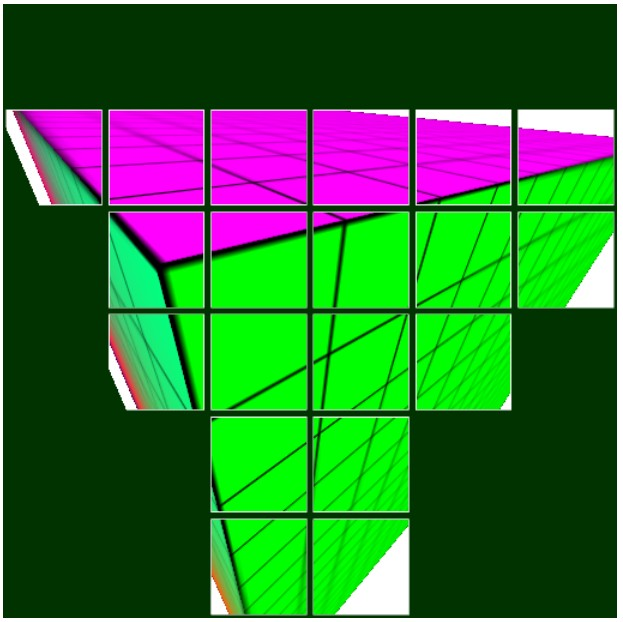
\includegraphics[width=.3\linewidth]{splat1.jpg}
  }
  \subfigure[$P_c M_c = P_s M_s$]{
    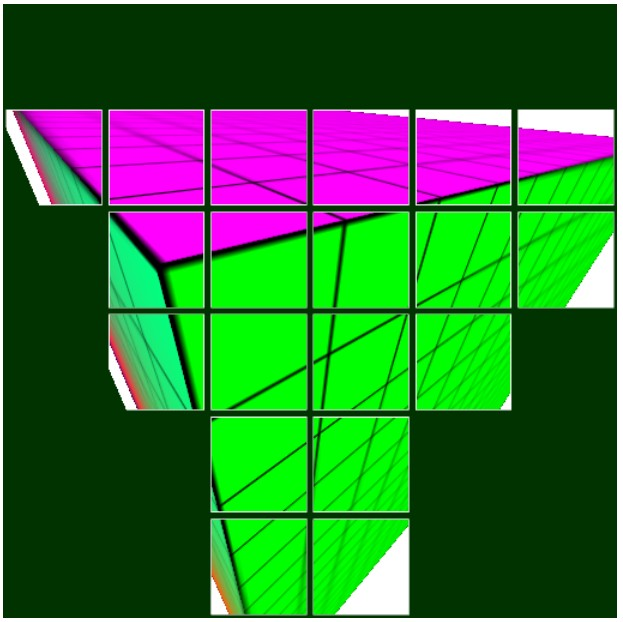
\includegraphics[width=.3\linewidth]{splat1.jpg}
  }
  \subfigure[$P_c M_c \neq P_s M_s$]{
    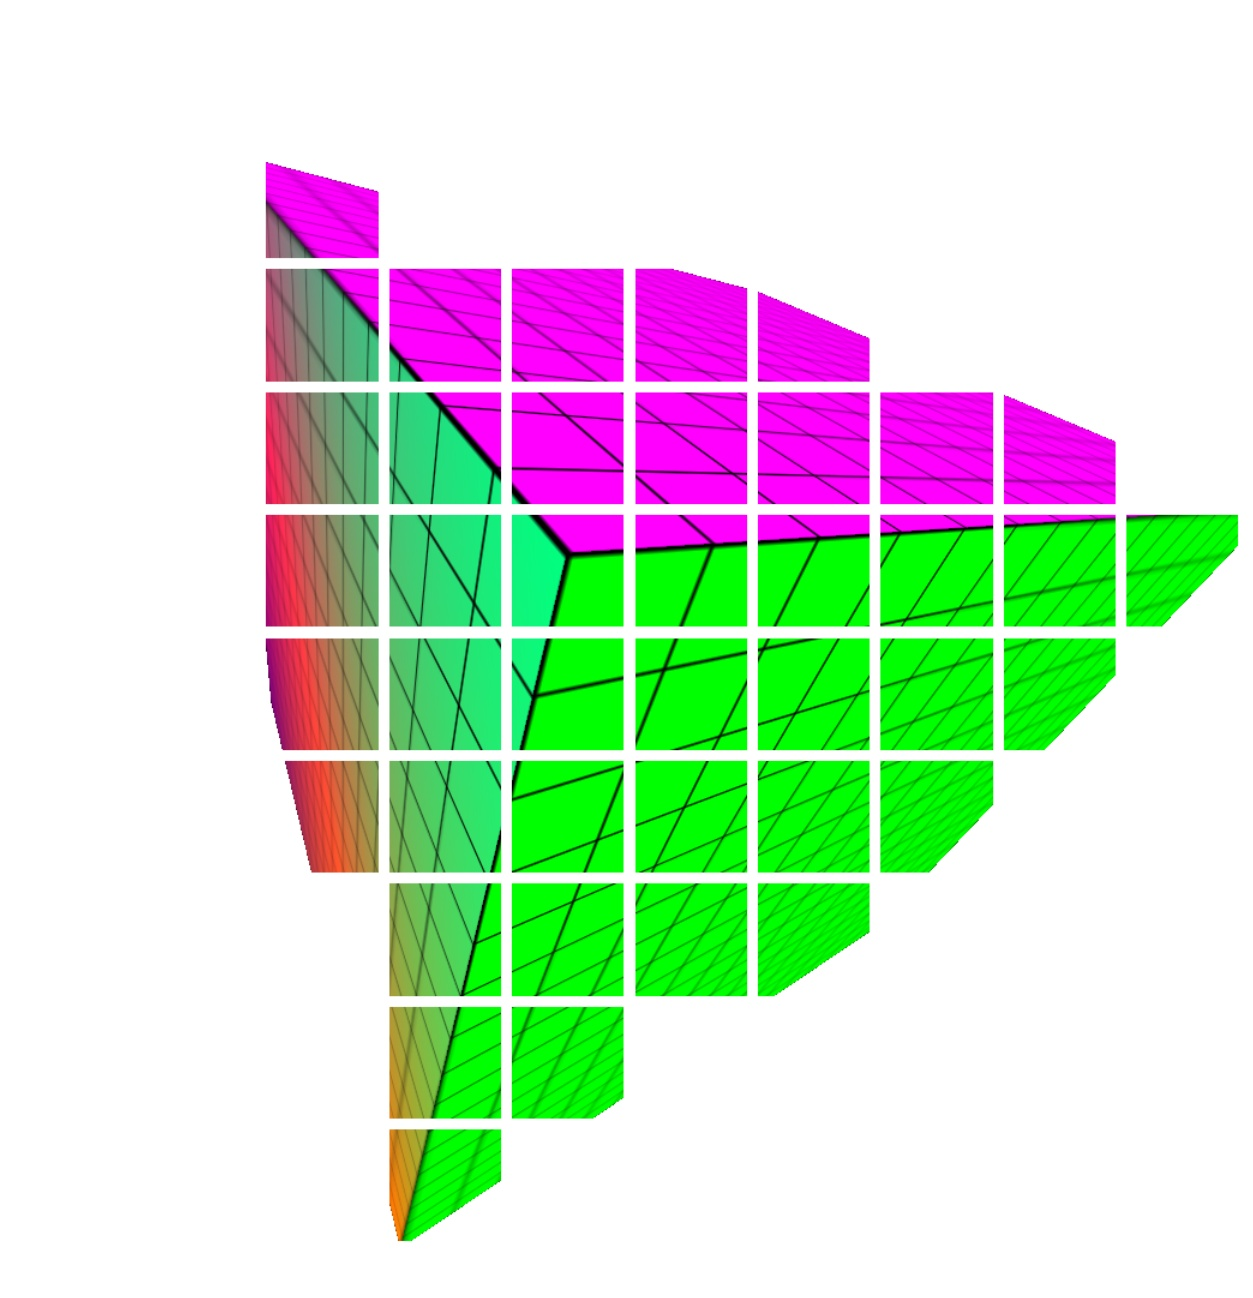
\includegraphics[width=.3\linewidth]{splat2.jpg}
  }
  \caption{\label{fig:LargeSplatsOnCorners}
           Splats for which depths are sampled on a planar region look nice on
  exactly this region, but contorted elsewhere, notice the corner of the cube.}
\end{figure}

The problem with this, is that the geometry is not planar, and our simple texture
coordinate transformation will produce the wrong result. Some ways to remedy
this, is to choose smaller (and more) splats, detect the problem and discard
such splats, or introduce more complex texture transformations. Since the proxy
geometry in principle is to be short-lived, and only a temporary geometry to be
rendered before the server-rendered image can be receieved, we have chosen the
first alternative. Discarding such splats may offer a good alternative,
especially when combining several proxy geometries, where the union of retained
splats increases the likelihood of all geometry parts being covered. Note also
that implementing a more sophisticated texture coordinate transformation may
actually amount to performing the same work as for more and smaller splats. Or,
in other words, using more and smaller splats may be regarded as a better
texture transform implementation.


%-------------------------------------------------------------------------
\subsubsection{Splat depth fragments}

For larger splats, covering many fragments, it makes sense to also compute and
use depth fragments. This will improve the usage of more proxy models
simultaneously, since the risk of a splat with a not very representative depth
value covers another and better splat is reduced. The ``intra-splat'' depth
values can easily be fetched from the depth image, just as the texture is looked
up for color. One problem is that many thin clients may not support this, in
WebGL, the ``frag depth'' feature is an extension, which may not be supported
everywhere.


%------------------------------------------------------------------------
\subsection{Splat set replacement algorithms}
\label{sec:proxyModelReplacement}

In this paper we concern ourselves with proxy models defined as sets of
splats. Since each splat set is the product of one instance of a server-rendered
image, depth buffer and viewing parameters, it makes sense to retain more than
one such model on the client. By doing this, the client may combine them, in
order to provide renderings for viewing parameters very different from the last
one received. One can imagine a plethora of splat set replacement algorithms, we
have tested two approaches which both works well; both retain a constant number
of proxy models. The first algorithm is to replace the one with a viewing
direction differing the most from the newly received model. The second simply
replaces the oldest one in store. The third replaces a proxy model $j$ if the
replacement results in the following objective function being reduced,
\[
  \text{coverage}_j = 
  \sum_{i=1, i\neq j}^n 
    \angle(\textbf{camdir}_i, \textbf{new camdir} )^2,
\]
where $\textbf{camdir}$ is the direction in which the camera was looking for the
generation of that particular proxy model.

There are some issues to consider with respect to panning and zooming that we
will not discuss here due to the limited space available.  All of these model
replacement algorithms work decently well.



%-------------------------------------------------------------------------
\subsection{Dynamic/heuristic method selection}

Since the main purpose of the automatically generated proxy model is to
facilitate a client-rendered image while waiting for one from the server for
increased interactivity, it is important that the process of generating and
sending proxy model data from the server itself is not hold up more than
necessary. There are mainly three sources of delay (\textbf{passer aa nevne
tidligere?}) for server-rendered images to the client; high
latency, low bandwidth, and slow server-rendering itself.

In the first case, it seems prudent to have a better proxy model on the client,
that can be used for longer time and for interactivity resulting in viewing
parameters deviating more from the last received server-rendered image. In the
two other cases, it is important for the proxy model generation/transmission to
be quicker, both in order to get the proxy model to the client and keep from
delaying the server-image more than necessary.

To take care of this, we have adopted an adaptive specification of
proxy model data from the server. This involves a more light-weight image (lossy
JPG-compression with adaptive quality control) while the user is interacting
with the client, as well as a reduced resolution of the depth buffer sent from
the server. See Figure~\ref{fig:adapativeProxyModels} for examples of low- and
high-quality proxy models.

\begin{figure}[htb]
  \centering
  \subfigure[Low quality (tenker her jpg med q=0 og daarlig dybdebuffer, faa
  splats kanskje]{
    %\begin{tikzpicture}[ scale=.25, show background rectangle]
\begin{tikzpicture}[scale=0.32, >=triangle 45, show background rectangle,
  declare function = {
    rotx(\x,\y,\th) = cos(\th)*\x - sin(\th)*\y; % NB! Cannot have space between parameters it seems!
    roty(\x,\y,\th) = sin(\th)*\x + cos(\th)*\y;
  }
  ]

  % View frustum
  \fill[fill=gray!20] (1, 0) -- (9, 0) -- (10, 5) -- (0, 5) -- cycle;
  % \clip (1, 0) -- (9, 0) -- (10, 5) -- (0, 5) -- cycle;
  % Clipping looks ok, but clipped content still expands bbox!! Solving this by reducing \pixels below from 13 to 11...


  % Defining some figure params

  \def \pixelwidth  {0.4}
  \def \pixelheight {0.3}
  \def \redstart    {2.2}
  \def \redpixels   {5}
  \def \pixels      {11}
  \def \linewidth   {1.25pt}
  \def \theta       {25}
  \def \cx          {5}
  \def \cy          {3}
  \def \rightcol    {red!100}
  \def \leftcolL    {blue!100}
  %\def \leftcolR    {red!100!blue!0} % Why doesn't this work?! (The color becomes white)
  \def \leftcolR    {red!100}


  % The scene, using same coordinate calculations as in the loop below

  \foreach \t in {0, ..., 4} {

    \pgfmathsetmacro\theta{25*\t}

    \ifthenelse{ \t = 0 \OR \t = 2 \OR \t = 4} {
      \def \rightcolToUse {\rightcol}
      \def \leftcolLToUse {\leftcolL}
      \def \leftcolRToUse {\leftcolR}
    }{
      \def \rightcolToUse {red!10}
      \def \leftcolLToUse {blue!10}
      \def \leftcolRToUse {red!10}
    }

    \pgfmathsetmacro\s{1}
    \pgfmathsetmacro\posx{0.5*(\s-1) + 2}
    \pgfmathsetmacro\posy{3.5 - 0.6*(\s-1)}
    \pgfmathsetmacro\posxRot{rotx(\posx-\cx, \posy-\cy, \theta)+\cx}
    \pgfmathsetmacro\posyRot{roty(\posx-\cx, \posy-\cy, \theta)+\cy}
    \coordinate (left) at ( \posxRot, \posyRot );
    
    \pgfmathsetmacro\s{\redpixels - 1}
    \pgfmathsetmacro\posx{0.5*(\s-1) + 2}
    \pgfmathsetmacro\posy{3.5 - 0.6*(\s-1)}
    \pgfmathsetmacro\posxRot{rotx(\posx-\cx, \posy-\cy, \theta)+\cx}
    \pgfmathsetmacro\posyRot{roty(\posx-\cx, \posy-\cy, \theta)+\cy}
    \coordinate (middle) at ( \posxRot, \posyRot );
    
    % The offset necessary for the red and green lines to meet properly
    \pgfmathsetmacro\redgreenintersection{3.5 -(0.6+0.2)*(\s-1)}
    
    \pgfmathsetmacro\s{\pixels}
    \pgfmathsetmacro\posx{0.5*(\s-1) + 2}
    \pgfmathsetmacro\posy{0.2*(\s-1) + \redgreenintersection}
    \pgfmathsetmacro\posxRot{rotx(\posx-\cx, \posy-\cy, \theta)+\cx}
    \pgfmathsetmacro\posyRot{roty(\posx-\cx, \posy-\cy, \theta)+\cy}
    \coordinate (right) at ( \posxRot, \posyRot );
    
    % The "server-rendered model"
    \fill[left color=\leftcolLToUse, right color=\leftcolRToUse, draw=none]
    (left) -- (middle) -- +(0, 3*\linewidth) -- ($ (left) + (0, 3*\linewidth) $) -- cycle;
    % Why is the factor 3 needed here?!?!
    % And why is there a (very thin) border?
    % And why is it not equally thick everywhere?

    \draw[\rightcolToUse, line width=\linewidth] (middle) -- (right);

  }


\end{tikzpicture}

  }
  \subfigure[High quality (png med maks av alt, mange splats)]{
    \begin{tikzpicture}[scale=0.32, >=triangle 45, show background rectangle,
  declare function = {
    rotx(\x,\y,\th) = cos(\th)*\x - sin(\th)*\y; % NB! Cannot have space between parameters it seems!
    roty(\x,\y,\th) = sin(\th)*\x + cos(\th)*\y;
  }
  ]

  % View frustum
  \fill[fill=gray!20] (1, 0) -- (9, 0) -- (10, 5) -- (0, 5) -- cycle;


  % Defining some figure params

  \def \pixelwidth  {0.4}
  \def \pixelheight {0.3}
  \def \redstart    {2.2}
  \def \redpixels   {5}
  \def \pixels      {11}
  \def \linewidth   {1.25pt}
  \def \cx          {5}
  \def \cy          {2.5}

  \pgfmathsetmacro\halfpixelwidth{0.5*\pixelwidth}


  \foreach \frame in {0} {  % , ..., 4} {
    \pgfmathsetmacro\theta{25*\frame}

    \ifthenelse{ \frame = 0 \OR \frame = 2 \OR \frame = 4} {
      \def \rightcolToUse {red!100}
      \def \leftcolLToUse {blue!100}
      \def \leftcolRToUse {red!100}
    }{
      \def \rightcolToUse {red!10}
      \def \leftcolLToUse {blue!10}
      \def \leftcolRToUse {red!10}
    }
    
    \def \withSplats {1}
    \def \withLargeSplats {0}
    \def \withConstantWidthSplats {1}
    \def \withFragDepth {0}

        \pgfmathsetmacro\s{1}
    \pgfmathsetmacro\posx{0.5*(\s-1) + 2}
    \pgfmathsetmacro\posy{3.5 - 0.6*(\s-1)}
    \pgfmathsetmacro\posxRot{rotx(\posx-\cx, \posy-\cy, 0)+\cx}
    \pgfmathsetmacro\posyRot{roty(\posx-\cx, \posy-\cy, 0)+\cy}
    \coordinate (left) at ( \posxRot, \posyRot );
    
    \pgfmathsetmacro\s{\redpixels - 1}
    \pgfmathsetmacro\posx{0.5*(\s-1) + 2}
    \pgfmathsetmacro\posy{3.5 - 0.6*(\s-1)}
    \pgfmathsetmacro\posxRot{rotx(\posx-\cx, \posy-\cy, 0)+\cx}
    \pgfmathsetmacro\posyRot{roty(\posx-\cx, \posy-\cy, 0)+\cy}
    \coordinate (middle) at ( \posxRot, \posyRot );
    
    % The offset necessary for the red and green lines to meet properly
    \pgfmathsetmacro\redgreenintersection{3.5 -(0.6+0.2)*(\s-1)}
    
    \pgfmathsetmacro\s{\pixels}
    \pgfmathsetmacro\posx{0.5*(\s-1) + 2}
    \pgfmathsetmacro\posy{0.2*(\s-1) + \redgreenintersection}
    \pgfmathsetmacro\posxRot{rotx(\posx-\cx, \posy-\cy, 0)+\cx}
    \pgfmathsetmacro\posyRot{roty(\posx-\cx, \posy-\cy, 0)+\cy}
    \coordinate (right) at ( \posxRot, \posyRot );
    
    % The "server-rendered model"
    \fill[left color=\leftcolLToUse, right color=\leftcolRToUse, draw=none]
      (left) -- (middle) -- +(0, 5*\linewidth) -- ($ (left) + (0, 5*\linewidth) $) -- cycle;
    % Why is the factor 3 needed here?!?!
    % And why is there a (very thin) border?
    % And why is it not equally thick everywhere?
    \draw[\rightcolToUse, line width=\linewidth] (middle) -- (right);

    \ifthenelse{ \withSplats = 1 } {
      \foreach \s in {1, ..., \pixels} {
        \ifthenelse{\s < \redpixels} {
          \pgfmathsetmacro\posx{0.5*(\s-1) + 2}
          \pgfmathsetmacro\posy{3.5 - 0.6*(\s-1)}
          \pgfmathsetmacro\posxRot{rotx(\posx-\cx, \posy-\cy, \theta)+\cx}
          \pgfmathsetmacro\posyRot{roty(\posx-\cx, \posy-\cy, \theta)+\cy}
          
          % Screen-space-sized splats
          \pgfmathsetmacro\posx{0.5*(\s-1-1) + 2}
          \pgfmathsetmacro\posy{3.5 - 0.6*(\s-1-1)}
          \pgfmathsetmacro\posxRotL{rotx(\posx-\cx, \posy-\cy, \theta)+\cx}
          \pgfmathsetmacro\posyRotL{roty(\posx-\cx, \posy-\cy, \theta)+\cy}
          \pgfmathsetmacro\posx{0.5*(\s-1) + 2}
          \pgfmathsetmacro\posy{3.5 - 0.6*(\s-1)}
          \pgfmathsetmacro\posxRotR{rotx(\posx-\cx, \posy-\cy, \theta)+\cx}
          \pgfmathsetmacro\posyRotR{roty(\posx-\cx, \posy-\cy, \theta)+\cy}
          \pgfmathsetmacro\halfWidthToUse{0.5*(\posxRotR-\posxRotL)}
          
          % Overriding with constant width for one of the sub-figures
          \ifthenelse{ \withConstantWidthSplats = 1 } {
            \pgfmathsetmacro\halfWidthToUse{\halfpixelwidth}
          }{}

          \ifthenelse{ \withLargeSplats = 1 } {
            % Varying color here on the left side
            \pgfmathsetmacro\tl{100*(\s-1)/\redpixels}
            \pgfmathsetmacro\ul{100-\tl)}
            \pgfmathsetmacro\tr{100*(\s  )/\redpixels}
            \pgfmathsetmacro\ur{100-\tr}
            \ifthenelse{ \withFragDepth = 0 } {
              \draw[left color=red!\tl!blue!\ul, right color=red!\tr!blue!\ur]
                (\posxRot-\halfWidthToUse, \posyRot) rectangle +(2*\halfWidthToUse, 0.2);
            }{
              % Tror kanskje at problemet med at ting kommer for langt til venstre her, skyldes at vi ser paa 
              % linjestykker fra s-1-1 til s-1. Burde muligens vaert fra s-1-0.5 til s-1+0.5?!
              % Replace with rotated rectangles, will probably look better...
              \draw[left color=red!\tl!blue!\ul, right color=red!\tr!blue!\ur]
                (\posxRotL, \posyRotL) -- (\posxRotR, \posyRotR) -- +(0, 5*\linewidth) -- 
                ($ (\posxRotL, \posyRotL) + (0, 5*\linewidth) $) -- cycle;
            }
          }{
            % Constant color, just a dot
            \pgfmathsetmacro\t{100*\s/\redpixels}
            \pgfmathsetmacro\u{100*(1.0-\s/\redpixels)}
            \draw[fill=red!\t!blue!\u] (\posxRot, \posyRot) circle(0.15);
          }
        } {
          \pgfmathsetmacro\posx{0.5*(\s-1) + 2}
          \pgfmathsetmacro\posy{0.2*(\s-1) + \redgreenintersection}
          \pgfmathsetmacro\posxRot{rotx(\posx-\cx, \posy-\cy, \theta)+\cx}
          \pgfmathsetmacro\posyRot{roty(\posx-\cx, \posy-\cy, \theta)+\cy}
          
          % Screen-space-sized splats
          \pgfmathsetmacro\posx{0.5*(\s-1-1) + 2}
          \pgfmathsetmacro\posy{0.2*(\s-1-1) + \redgreenintersection}
          \pgfmathsetmacro\posxRotL{rotx(\posx-\cx, \posy-\cy, \theta)+\cx}
          \pgfmathsetmacro\posyRotL{roty(\posx-\cx, \posy-\cy, \theta)+\cy}
          \pgfmathsetmacro\posx{0.5*(\s-1) + 2}
          \pgfmathsetmacro\posy{0.2*(\s-1) + \redgreenintersection}
          \pgfmathsetmacro\posxRotR{rotx(\posx-\cx, \posy-\cy, \theta)+\cx}
          \pgfmathsetmacro\posyRotR{roty(\posx-\cx, \posy-\cy, \theta)+\cy}
          \pgfmathsetmacro\halfWidthToUse{0.5*(\posxRotR-\posxRotL)}
          
          \ifthenelse{ \withConstantWidthSplats = 1 } {
            % Overriding with constant width for one of the sub-figures
            \pgfmathsetmacro\halfWidthToUse{\halfpixelwidth}
          }{}

          \ifthenelse{ \withLargeSplats = 1 } {
            \ifthenelse{ \withFragDepth = 0 } {
              \draw[fill=\rightcolToUse]
                (\posxRot-\halfWidthToUse, \posyRot) rectangle +(2*\halfWidthToUse, 0.2);
            }{
              % \draw[fill=\rightcolToUse, line width=1.5pt] (\posxRotL, \posyRotL) -- (\posxRotR, \posyRotR);
              % Tror kanskje at problemet med at ting kommer for langt til venstre her, skyldes at vi ser paa 
              % linjestykker fra s-1-1 til s-1. Burde muligens vaert fra s-1-0.5 til s-1+0.5?!
              % Replace with rotated rectangles, will probably look better...
              \draw[fill=\rightcolToUse]
                (\posxRotL, \posyRotL) -- (\posxRotR, \posyRotR) -- +(0, 5*\linewidth) -- 
                ($ (\posxRotL, \posyRotL) + (0, 5*\linewidth) $) -- cycle;
            }
          }{
            % Constant color, just a dot
            \draw[fill=\rightcolToUse] (\posxRot, \posyRot) circle(0.15);
          }
        }
      }
    }{}

    
  }


\end{tikzpicture}

  }
  \caption{\label{fig:adapativeProxyModels}
           Proxy models adaptively adjusted to available bandwidth and server
           capacity.}
\end{figure}



%-------------------------------------------------------------------------
\section{Results and discussion}

We have tested the algorithms discussed in the Tinia framework, which is a
programming framework for setting up and managing a client/server based
interactive OpenGL-based visualization application. The client is
Javascript/WebGL-based and runs in one of several possible browsers, \eg Chrome
or Firefox. This client communicates over tcp/ip, using either http or
websockets, with a server running as an Apache module.

The automatic proxy geometry implementation is fully invisible to the
application, meaning that all existing applications immediately will have the
feature available. We have tested the algorithm on several smaller test cases,
but also on a larger oild reservoir viewer.

This viewer utilizes several GLSL shaders to render reservoir cells and
boundaries, tubular wells etc., and operates in general on a geometric model
that is not trivial to reduce in complexity. The model is typically also very
large, meaning that rendering on a thin client is prohibitive. With the
automatic proxy geometry, we can obtain interactive frame rates with a bad
connection from a very lightweight client to the server. For a comparison of a
server-rendered image and a client-rendered proxy model, see
Figure~\ref{fig:FRView}.

\begin{figure}[htb]
  \centering
  \subfigure[Server-rendered]{
    %\begin{tikzpicture}[ scale=.25, show background rectangle]
\begin{tikzpicture}[scale=0.32, >=triangle 45, show background rectangle,
  declare function = {
    rotx(\x,\y,\th) = cos(\th)*\x - sin(\th)*\y; % NB! Cannot have space between parameters it seems!
    roty(\x,\y,\th) = sin(\th)*\x + cos(\th)*\y;
  }
  ]

  % View frustum
  \fill[fill=gray!20] (1, 0) -- (9, 0) -- (10, 5) -- (0, 5) -- cycle;
  % \clip (1, 0) -- (9, 0) -- (10, 5) -- (0, 5) -- cycle;
  % Clipping looks ok, but clipped content still expands bbox!! Solving this by reducing \pixels below from 13 to 11...


  % Defining some figure params

  \def \pixelwidth  {0.4}
  \def \pixelheight {0.3}
  \def \redstart    {2.2}
  \def \redpixels   {5}
  \def \pixels      {11}
  \def \linewidth   {1.25pt}
  \def \theta       {25}
  \def \cx          {5}
  \def \cy          {3}
  \def \rightcol    {red!100}
  \def \leftcolL    {blue!100}
  %\def \leftcolR    {red!100!blue!0} % Why doesn't this work?! (The color becomes white)
  \def \leftcolR    {red!100}


  % The scene, using same coordinate calculations as in the loop below

  \foreach \t in {0, ..., 4} {

    \pgfmathsetmacro\theta{25*\t}

    \ifthenelse{ \t = 0 \OR \t = 2 \OR \t = 4} {
      \def \rightcolToUse {\rightcol}
      \def \leftcolLToUse {\leftcolL}
      \def \leftcolRToUse {\leftcolR}
    }{
      \def \rightcolToUse {red!10}
      \def \leftcolLToUse {blue!10}
      \def \leftcolRToUse {red!10}
    }

    \pgfmathsetmacro\s{1}
    \pgfmathsetmacro\posx{0.5*(\s-1) + 2}
    \pgfmathsetmacro\posy{3.5 - 0.6*(\s-1)}
    \pgfmathsetmacro\posxRot{rotx(\posx-\cx, \posy-\cy, \theta)+\cx}
    \pgfmathsetmacro\posyRot{roty(\posx-\cx, \posy-\cy, \theta)+\cy}
    \coordinate (left) at ( \posxRot, \posyRot );
    
    \pgfmathsetmacro\s{\redpixels - 1}
    \pgfmathsetmacro\posx{0.5*(\s-1) + 2}
    \pgfmathsetmacro\posy{3.5 - 0.6*(\s-1)}
    \pgfmathsetmacro\posxRot{rotx(\posx-\cx, \posy-\cy, \theta)+\cx}
    \pgfmathsetmacro\posyRot{roty(\posx-\cx, \posy-\cy, \theta)+\cy}
    \coordinate (middle) at ( \posxRot, \posyRot );
    
    % The offset necessary for the red and green lines to meet properly
    \pgfmathsetmacro\redgreenintersection{3.5 -(0.6+0.2)*(\s-1)}
    
    \pgfmathsetmacro\s{\pixels}
    \pgfmathsetmacro\posx{0.5*(\s-1) + 2}
    \pgfmathsetmacro\posy{0.2*(\s-1) + \redgreenintersection}
    \pgfmathsetmacro\posxRot{rotx(\posx-\cx, \posy-\cy, \theta)+\cx}
    \pgfmathsetmacro\posyRot{roty(\posx-\cx, \posy-\cy, \theta)+\cy}
    \coordinate (right) at ( \posxRot, \posyRot );
    
    % The "server-rendered model"
    \fill[left color=\leftcolLToUse, right color=\leftcolRToUse, draw=none]
    (left) -- (middle) -- +(0, 3*\linewidth) -- ($ (left) + (0, 3*\linewidth) $) -- cycle;
    % Why is the factor 3 needed here?!?!
    % And why is there a (very thin) border?
    % And why is it not equally thick everywhere?

    \draw[\rightcolToUse, line width=\linewidth] (middle) -- (right);

  }


\end{tikzpicture}

  }
  \subfigure[Client-rendered proxy model]{
    \begin{tikzpicture}[scale=0.32, >=triangle 45, show background rectangle,
  declare function = {
    rotx(\x,\y,\th) = cos(\th)*\x - sin(\th)*\y; % NB! Cannot have space between parameters it seems!
    roty(\x,\y,\th) = sin(\th)*\x + cos(\th)*\y;
  }
  ]

  % View frustum
  \fill[fill=gray!20] (1, 0) -- (9, 0) -- (10, 5) -- (0, 5) -- cycle;


  % Defining some figure params

  \def \pixelwidth  {0.4}
  \def \pixelheight {0.3}
  \def \redstart    {2.2}
  \def \redpixels   {5}
  \def \pixels      {11}
  \def \linewidth   {1.25pt}
  \def \cx          {5}
  \def \cy          {2.5}

  \pgfmathsetmacro\halfpixelwidth{0.5*\pixelwidth}


  \foreach \frame in {0} {  % , ..., 4} {
    \pgfmathsetmacro\theta{25*\frame}

    \ifthenelse{ \frame = 0 \OR \frame = 2 \OR \frame = 4} {
      \def \rightcolToUse {red!100}
      \def \leftcolLToUse {blue!100}
      \def \leftcolRToUse {red!100}
    }{
      \def \rightcolToUse {red!10}
      \def \leftcolLToUse {blue!10}
      \def \leftcolRToUse {red!10}
    }
    
    \def \withSplats {1}
    \def \withLargeSplats {0}
    \def \withConstantWidthSplats {1}
    \def \withFragDepth {0}

        \pgfmathsetmacro\s{1}
    \pgfmathsetmacro\posx{0.5*(\s-1) + 2}
    \pgfmathsetmacro\posy{3.5 - 0.6*(\s-1)}
    \pgfmathsetmacro\posxRot{rotx(\posx-\cx, \posy-\cy, 0)+\cx}
    \pgfmathsetmacro\posyRot{roty(\posx-\cx, \posy-\cy, 0)+\cy}
    \coordinate (left) at ( \posxRot, \posyRot );
    
    \pgfmathsetmacro\s{\redpixels - 1}
    \pgfmathsetmacro\posx{0.5*(\s-1) + 2}
    \pgfmathsetmacro\posy{3.5 - 0.6*(\s-1)}
    \pgfmathsetmacro\posxRot{rotx(\posx-\cx, \posy-\cy, 0)+\cx}
    \pgfmathsetmacro\posyRot{roty(\posx-\cx, \posy-\cy, 0)+\cy}
    \coordinate (middle) at ( \posxRot, \posyRot );
    
    % The offset necessary for the red and green lines to meet properly
    \pgfmathsetmacro\redgreenintersection{3.5 -(0.6+0.2)*(\s-1)}
    
    \pgfmathsetmacro\s{\pixels}
    \pgfmathsetmacro\posx{0.5*(\s-1) + 2}
    \pgfmathsetmacro\posy{0.2*(\s-1) + \redgreenintersection}
    \pgfmathsetmacro\posxRot{rotx(\posx-\cx, \posy-\cy, 0)+\cx}
    \pgfmathsetmacro\posyRot{roty(\posx-\cx, \posy-\cy, 0)+\cy}
    \coordinate (right) at ( \posxRot, \posyRot );
    
    % The "server-rendered model"
    \fill[left color=\leftcolLToUse, right color=\leftcolRToUse, draw=none]
      (left) -- (middle) -- +(0, 5*\linewidth) -- ($ (left) + (0, 5*\linewidth) $) -- cycle;
    % Why is the factor 3 needed here?!?!
    % And why is there a (very thin) border?
    % And why is it not equally thick everywhere?
    \draw[\rightcolToUse, line width=\linewidth] (middle) -- (right);

    \ifthenelse{ \withSplats = 1 } {
      \foreach \s in {1, ..., \pixels} {
        \ifthenelse{\s < \redpixels} {
          \pgfmathsetmacro\posx{0.5*(\s-1) + 2}
          \pgfmathsetmacro\posy{3.5 - 0.6*(\s-1)}
          \pgfmathsetmacro\posxRot{rotx(\posx-\cx, \posy-\cy, \theta)+\cx}
          \pgfmathsetmacro\posyRot{roty(\posx-\cx, \posy-\cy, \theta)+\cy}
          
          % Screen-space-sized splats
          \pgfmathsetmacro\posx{0.5*(\s-1-1) + 2}
          \pgfmathsetmacro\posy{3.5 - 0.6*(\s-1-1)}
          \pgfmathsetmacro\posxRotL{rotx(\posx-\cx, \posy-\cy, \theta)+\cx}
          \pgfmathsetmacro\posyRotL{roty(\posx-\cx, \posy-\cy, \theta)+\cy}
          \pgfmathsetmacro\posx{0.5*(\s-1) + 2}
          \pgfmathsetmacro\posy{3.5 - 0.6*(\s-1)}
          \pgfmathsetmacro\posxRotR{rotx(\posx-\cx, \posy-\cy, \theta)+\cx}
          \pgfmathsetmacro\posyRotR{roty(\posx-\cx, \posy-\cy, \theta)+\cy}
          \pgfmathsetmacro\halfWidthToUse{0.5*(\posxRotR-\posxRotL)}
          
          % Overriding with constant width for one of the sub-figures
          \ifthenelse{ \withConstantWidthSplats = 1 } {
            \pgfmathsetmacro\halfWidthToUse{\halfpixelwidth}
          }{}

          \ifthenelse{ \withLargeSplats = 1 } {
            % Varying color here on the left side
            \pgfmathsetmacro\tl{100*(\s-1)/\redpixels}
            \pgfmathsetmacro\ul{100-\tl)}
            \pgfmathsetmacro\tr{100*(\s  )/\redpixels}
            \pgfmathsetmacro\ur{100-\tr}
            \ifthenelse{ \withFragDepth = 0 } {
              \draw[left color=red!\tl!blue!\ul, right color=red!\tr!blue!\ur]
                (\posxRot-\halfWidthToUse, \posyRot) rectangle +(2*\halfWidthToUse, 0.2);
            }{
              % Tror kanskje at problemet med at ting kommer for langt til venstre her, skyldes at vi ser paa 
              % linjestykker fra s-1-1 til s-1. Burde muligens vaert fra s-1-0.5 til s-1+0.5?!
              % Replace with rotated rectangles, will probably look better...
              \draw[left color=red!\tl!blue!\ul, right color=red!\tr!blue!\ur]
                (\posxRotL, \posyRotL) -- (\posxRotR, \posyRotR) -- +(0, 5*\linewidth) -- 
                ($ (\posxRotL, \posyRotL) + (0, 5*\linewidth) $) -- cycle;
            }
          }{
            % Constant color, just a dot
            \pgfmathsetmacro\t{100*\s/\redpixels}
            \pgfmathsetmacro\u{100*(1.0-\s/\redpixels)}
            \draw[fill=red!\t!blue!\u] (\posxRot, \posyRot) circle(0.15);
          }
        } {
          \pgfmathsetmacro\posx{0.5*(\s-1) + 2}
          \pgfmathsetmacro\posy{0.2*(\s-1) + \redgreenintersection}
          \pgfmathsetmacro\posxRot{rotx(\posx-\cx, \posy-\cy, \theta)+\cx}
          \pgfmathsetmacro\posyRot{roty(\posx-\cx, \posy-\cy, \theta)+\cy}
          
          % Screen-space-sized splats
          \pgfmathsetmacro\posx{0.5*(\s-1-1) + 2}
          \pgfmathsetmacro\posy{0.2*(\s-1-1) + \redgreenintersection}
          \pgfmathsetmacro\posxRotL{rotx(\posx-\cx, \posy-\cy, \theta)+\cx}
          \pgfmathsetmacro\posyRotL{roty(\posx-\cx, \posy-\cy, \theta)+\cy}
          \pgfmathsetmacro\posx{0.5*(\s-1) + 2}
          \pgfmathsetmacro\posy{0.2*(\s-1) + \redgreenintersection}
          \pgfmathsetmacro\posxRotR{rotx(\posx-\cx, \posy-\cy, \theta)+\cx}
          \pgfmathsetmacro\posyRotR{roty(\posx-\cx, \posy-\cy, \theta)+\cy}
          \pgfmathsetmacro\halfWidthToUse{0.5*(\posxRotR-\posxRotL)}
          
          \ifthenelse{ \withConstantWidthSplats = 1 } {
            % Overriding with constant width for one of the sub-figures
            \pgfmathsetmacro\halfWidthToUse{\halfpixelwidth}
          }{}

          \ifthenelse{ \withLargeSplats = 1 } {
            \ifthenelse{ \withFragDepth = 0 } {
              \draw[fill=\rightcolToUse]
                (\posxRot-\halfWidthToUse, \posyRot) rectangle +(2*\halfWidthToUse, 0.2);
            }{
              % \draw[fill=\rightcolToUse, line width=1.5pt] (\posxRotL, \posyRotL) -- (\posxRotR, \posyRotR);
              % Tror kanskje at problemet med at ting kommer for langt til venstre her, skyldes at vi ser paa 
              % linjestykker fra s-1-1 til s-1. Burde muligens vaert fra s-1-0.5 til s-1+0.5?!
              % Replace with rotated rectangles, will probably look better...
              \draw[fill=\rightcolToUse]
                (\posxRotL, \posyRotL) -- (\posxRotR, \posyRotR) -- +(0, 5*\linewidth) -- 
                ($ (\posxRotL, \posyRotL) + (0, 5*\linewidth) $) -- cycle;
            }
          }{
            % Constant color, just a dot
            \draw[fill=\rightcolToUse] (\posxRot, \posyRot) circle(0.15);
          }
        }
      }
    }{}

    
  }


\end{tikzpicture}

  }
  \caption{\label{fig:FRView}
           The oil reservoir viewer FRView}
\end{figure}


%-------------------------------------------------------------------------
\section{Conclusion and future work}

The single most attractive feature of such an automatic proxy geometry as
described, is exactly the automated generation. It means that problems with
downscaling, sending and rendering existing geometries is bypassed
altogether. The Tinia framework with which we have demonstrated this, is a
framework for setting up and managing a client/server based interactive OpenGL
based visualization application. The automatic proxy geometry implementation is
fully invisible to the application, meaning that all existing applications
immediately will have the feature available.

There are several directions in which we would like to follow up and improve
this concept,
\begin{itemize}
\item \textbf{Proxy model replacement algorithms} The goal is to obtain a good view with
all relevant viewing parameters on the client, with the help of a minimal set of
proxy models.
\item \textbf{Grid-based proxy geometry} Instead of a set of ``splats'', one can
envision a spatially partioned grid, for instance containing a distance field,
with the geometry as an iso-surface.
\end{itemize}




%-------------------------------------------------------------------------

%\bibliographystyle{eg-alpha}
\bibliographystyle{eg-alpha-doi}

\bibliography{egbibsample}

%-------------------------------------------------------------------------

\end{document}
